\documentclass{VUMIFInfBakalaurinis}
\usepackage{algorithmicx}
\usepackage{algorithm}
\usepackage{algpseudocode}
\usepackage{amsfonts}
\usepackage{amsmath}
\usepackage{bm}
\usepackage{caption}
\usepackage{color}
\usepackage{float}
\usepackage{graphicx}
% \usepackage{hyperref}  % Nuorodų aktyvavimas
\usepackage{listings}
\usepackage{subfig}
\usepackage{url}
\usepackage{wrapfig}
\usepackage{adjustbox}
%\usepackage{csquotes}
%\usepackage[autostyle,german=guillemets,norwegian=quotes]{csquotes}
\usepackage{dirtytalk}

\usepackage[utf8]{inputenc}
\usepackage[english,lithuanian]{babel}

% Titulinio aprašas
\university{Vilniaus universitetas}
\faculty{Matematikos ir informatikos fakultetas}
\department{Programų sistemų studijų programa}
\papertype{Baigiamasis bakalauro darbas}
\title{Privačios informacijos išsaugojimas taikant dirbtinio intelekto technologijas}
\titleineng{Privacy-preserving artificial intelligence}
\status{4 kurso 3 grupės studentas}
\author{Paulius Milmantas}
\supervisor{Dr. Linas Petkevičius}
\reviewer{Dr. Tomas Plankis}
\date{Vilnius \\ \the\year}

% Nustatymai


\begin{document}
\maketitle

\tableofcontents

\sectionnonum{Įvadas}
	%(https://eur-lex.europa.eu/legal-content/LT/TXT/?uri=celex%3A32016R0679)	
	\par Mašininis mokymas yra dirbtinio intelekto sritis, kuri pasitelkia statistinius algoritmus, kad apibrėžtų duomenų generavimo mechanizmą, ar egzistuojančius sąryšius, priklausomybes. Modelis dažnai turi didelį kiekį nežinomų parametrų, kuriuos reikia įvertinti iš duomenų, todėl modelio apmokymui dažniausiai reikia turėti daug duomenų. Kai kurie uždaviniai reikalauja duomenų, kurie nėra laisvai prieinami ir yra privatūs. Mašininio mokymo tyrimų srityje yra kilusi problema dėl jų saugojimo \cite{10}. Vienas iš faktorių, kuris lėmė šį susidomėjimą yra 2016 metais Europos Sąjungoje priimtas duomenų apsaugos reglamentas (GDPR). Pagal jį, fizinių asmenų duomenys turi būti saugomi naudojantis tam tikromis taisyklėmis ir negali būti atskleisti trečiosioms šalims, be asmens sutikimo \cite{1}.
	% https://towardsdatascience.com/perfectly-privacy-preserving-ai-c14698f322f5
	\par Šią problemą išspręsti siekia įvairūs tyrimai ir naujai pasiūlyti metodai privatumą saugančio dirbtinio intelekto srityje. Šią problemą galima išskaidyti į kelias atskiras sritis:
\begin{itemize}
    \item Analizuojamų duomenų privatumas \cite{2}. Algoritmas apmoko modelį atpažinti duomenis. Turint sukurtą modelį, neturi būti galima atgaminti duomenų, pagal kuriuos jis buvo mokomas, bei negali būti identifikuoti asmenys. Taip nukentėtų žmonių privatumas ir būtų pažeistas Europos duomenų apsaugos reglamentas. Šio pažeidimo pavyzdys gali būti ir paprastas teksto atkūrimo modelis. Duodama sakinio pradžia, modelis nuspėja jo pabaigą. Jeigu suvedus tam tikras detales modelis užbaigia sakinį naudodamas asmeninius duomenis, kurie atskleidžia žmonių tapatybę, šis modelis nėra saugus \cite{12}.
    \item Duomenų įvesties privatumas. Trečios šalys neturi matyti įvedamų duomenų. Tai gali būti tinklo saugumo spragos, duomenų surinkimo aplikacijų spragos ir t.t…
    \item Modelio išvesties privatumas. Modelio išvesties neturi matyti asmenys, kuriems šie duomenys nepriklauso. Šis punktas yra sąlyginis, priklauso nuo modelio svarbos. Jeigu tai yra svarbūs asmeniniai duomenys, negalima rizikuoti. Tačiau jeigu tai yra viešai prieinami duomenys, šis punktas negalioja.
    \item Modelio apsauga. Sukurtas modelis negali būti niekieno pasisavintas. Šis punktas yra skirtas apsaugoti programos kūrėją.
\end{itemize}

	% https://www.nature.com/articles/s42256-020-0186-1 [Nepanaudotas]
	% https://towardsdatascience.com/the-new-dawn-of-ai-federated-learning-8ccd9ed7fc3a
	\par Darbo tikslas - ištirti ir palyginti privatumą saugančius dirbtinio intelekto algoritmus pagal jų saugumą, našumą ir panaudojamumą, bei pateikti rekomendacijas.
	\par Darbo uždaviniai:
	\begin{itemize}
		\item Išanalizuoti esamus algoritmus pagal jų saugumą ir panaudojamumą.
		\item Identifikuoti kriterijus, kurių pagalba galima įvertinti privatumo išsaugojimą, bei palyginti algoritmus tarpusavyje.
		\item Ištirti kurie algoritmai yra realizuoti realizuoti algoritmus, kurie nėra atvirai prieinami.
		\item Palyginti algoritmus pagal našumą ir pateikti rekomendacijas.
	\end{itemize}
\section{Asmens duomenų privatumas mašininio mokymo kontekste}
	\par Vienas iš būdų apsaugoti duomenis yra decentralizuoti modelį ir naudoti paskirstyto mokymo algoritmus. Paprastai mašininiam mokymui yra naudojamas centralizuotas serveris. Yra surenkami duomenys į vieną vietą ir modelį moko vienas kompiuteris. Jeigu norima pridėti daugiau duomenų arba papildomą klasifikatorių, modelį reikia apmokyti iš naujo. Taip pat, kas kuria šį modelį, turi visą prieigą prie duomenų, šie modeliai nėra saugūs \cite{13}. 
	\par Šiai bėdai išspręsti, vienas iš metodų yra federuotas mašininis mokymas (\say{Federated machine learning}). Šis metodas padeda išspręsti kai kurias bėdas, vykdant modelio mokymą decentralizuotai \cite{3}. Prie bendro tinklo gali prisijungti daug įrenginių. Visi jie turi savo unikalų duomenų rinkinį. Kiekvienas įrenginys pasirenka geriausią statistinį metodą modelio mokymui ir pagal tą metodą sukuria modelį. Taip yra sukuriama daug skirtingų modelių, realizuotų su skirtingais duomenų rinkiniais. Visi šie rinkiniai vėliau yra surenkami į vieną vietą ir toliau naudojami duomenų analizei. Taip surinkus atskirų įrenginių sukurtus modelius, neturime prieigos prie pradinių duomenų ir daugiau žmonių gali prisidėti prie modelio kūrimo, nematant pilno duomenų rinkinio. Tačiau naudojant šį metodą ne visos problemos yra išsprendžiamos. Duomenų saugumas nėra garantuojamas \cite{3}. Jeigu duomenys nėra užšifruojami, jie gali būti pavogti. Tai gali būti padaryta, jeigu yra naudojamas nesaugus interneto ryšys, arba jeigu yra bandoma analizuoti atskirų įrenginių atsiųstus modelius. Šis metodas išsprendžia tik kelias problemas. Likusios yra: komunikavimo kaštai, įrenginių heterogeniškumas, statistinis heterogeniškumas ir saugumo problemos \cite{4}.
%https://www.researchgate.net/publication/335319008_Federated_Learning_Challenges_Methods_and_Future_Directions [Nepanaudotas]
	\par Visos šios problemos yra nagrinėjamos ir joms spręsti kuriami nauji metodai. Komunikacijos kaštams mažinti, yra kuriami algoritmai, kaip turi būti perduodamas modelis tinkle, kad būtų maža tinklo apkrova. Įrenginių heterogeniškumui spręsti, yra parenkami tam tikri įrenginių rodikliai ir pagal tai nustatoma, kokia bus įrenginio komunikacija: ar jis naudos asinchroninį komunikavimą, kaip dažnai tai vyks ir kokia yra įrenginio klaidos tikimybė \cite{4}. Statistikos heterogeniškumui pataisyti kuriami yra metodai, kaip meta duomenų-mokymas ir keletos užduočių mokymas (\say{Multi-task learning}). 
	% https://arxiv.org/pdf/1906.10893.pdfmif
	\par Straipsnyje apie privatumą išsaugančius blokų-grandinių tinklus (\say{Privacy-Preserving Blockchain-Based Federated Learning for IoT Devices}) yra pateikiamas naujas paskirstyto mokymosi algoritmas, kuris yra paremtas
blokų grandinių technologijomis \cite{5}. Šis modelis yra grafiškai pateiktas pav.1. Šią architektūrą pavyzdyje sudaro 3 komponentai: gamintojai, klientai ir blokų grandinių tinklas. Šiame pavyzdyje gamintojas pareiškia užklausą, kad reikia atlikti apklausą. Klientai, kurie sutinka su užklausa, išsiunčia savo sukurtą modelį. Blokų grandinių tinklas elgiasi kaip centralizuotas serveris ir surenka visus klientų modelius. Tuomet, pasirinktas kompiuteris, kuris atlieka visą darbą (\say{miner}) atlieka galutinį modelių sujungimą.

\begin{figure}[ht]
  \centering
  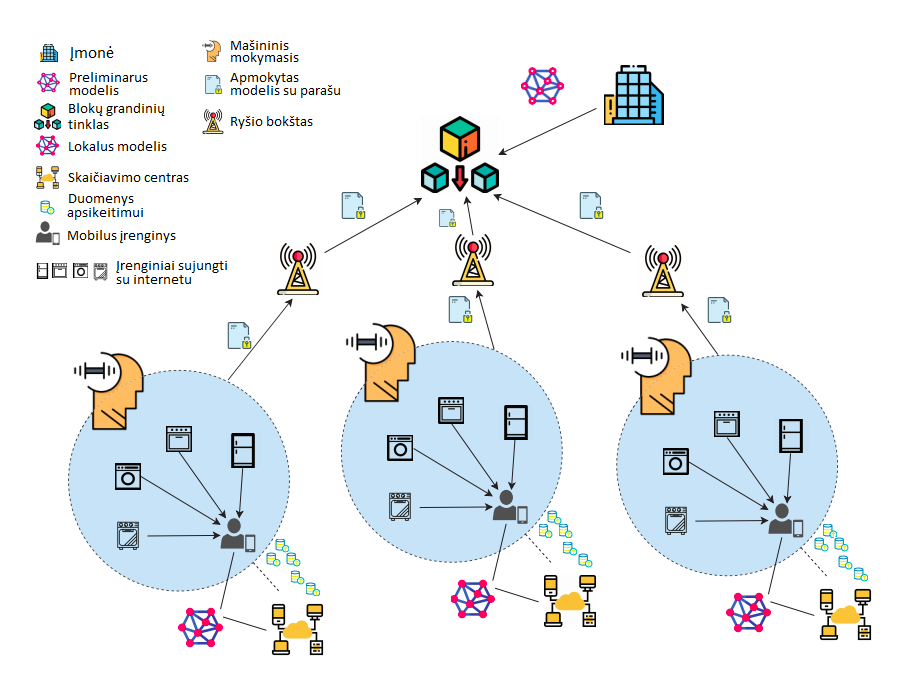
\includegraphics[width=13cm,height=11cm,keepaspectratio]{img/paskirstytasMokymasis.png}
  \caption{Paskirstytas mokymas \cite{5}}
  \label{fig:overflowProblem}
\end{figure}

% https://www.inpher.io/technology/what-is-secure-multiparty-computation
\par Minėti decentralizuoti būdai apjungia skirtingus sukurtus modelius į vieną ir visi įrenginiai kurie kuria modelius, naudoja savo unikalius duomenis. Saugus skirtingų pusių skaičiavimo metodas (\say{Secure multiparty computation}) yra kriptografinis protokolas, kuris leidžia įrenginiams, su unikaliais duomenimis, skaičiuoti funkcijos reikšmę, nematant kitų įrenginių reikšmių \cite{6}. Su šiuo metodu, yra sukuriamas vienas modelis tarp įvairių įrenginių. Pagrindinis įrenginys, kuris ruošia skaičiavimo užklausą, gali suskaidyti pradinius duomenis, užšifruoti juos ir taip paskirstyti tarp kitų įrenginių. Taip sukurti įrenginio rezultatai negali būti atšifruoti ir pasisavinti, o minėto federuoto mokymo metodo sukurti rezultatai, jeigu nėra gerai apsaugoti, gali būti pasisavinti ir atgauti pradiniai duomenys su kuriais modelis buvo sukurtas.
% https://www.researchgate.net/publication/236935821_Homomorphic_Encryption_Theory_Applications
\par  Kitas būdas apsaugoti modelį yra naudoti homomorfinį šifravimą. Pagal šį metodas, modelis yra mokomas naudojant užšifruotais duomenimis. Jie mokymo metu, nėra atšifruojami. Šis metodas leidžia keliems įrenginiams vienu metu atlikti skaičiavimus su duomenimis, kurių jie nemato. Yra daug metodo varijacijų. Kai kurios yra pažeidžiamos ir gali atskleisti visos infrastruktūros duomenis \cite{7}. Dažniausiai homomorfinės sistemos yra labiau pažeidžiamos nei nehomomorfinės.
% https://eprint.iacr.org/2016/421.pdf
\par 2016 metais buvo pasiūlytas naujas metodas paspartinti pilnai homomorfines šifravimo sistemas \cite{8}. Homomorfinės sistemos, kurios naudoja šį metodą yra laikomos ketvirtos kartos. Šis metodas leidžia aproksimuoti užšifruoto teksto sudėtį, daugybą ir pakeisti atšifruoto teksto proporcijas. 
Proporcijų pakeitimo procedūra suskaido užšifruotą tekstą į dalis, to pasekoje yra apvalinamas neužšifruotas tekstas. Šio metodo pagrindinė idėja yra pridėti triukšmo prie pagrindinės žinutės. Šis triukšmas yra pridedamas prie neužšifruoto teksto dėl saugumo priežasčių ir jis yra laikomas kaip aproksimavimo paklaida. Tuo pasekoje, metodas veikia su tam tikra paklaida
% https://www.inpher.io/technology/what-is-secure-multiparty-computation
\par Bendro įspūdžio agregavimo metodas yra naujausias iš visų minėtų. Jis leidžia įrenginiui su savo duomenimis sukurti modelį naudojant bet kokius metodus ir taip prisidėti prie bendro progreso \cite{6}. Visi modeliai yra surenkami ir leidžiami duomenys per šiuos modelius. Kiekvienas modelis skiria savo balsą, jie surenkami ir padaromas bendras sprendimas. Šis metodas leidžia lengvai plėsti modelį. Taip pat yra saugomas ir duomenų privatumas. Jeigu keli modeliai, kurie nesidalina duomenimis, teigia vienodai, tai reiškia, kad negalima atkurti duomenų ir jie yra saugūs. Skaičiavimas vykdomas pasirenkant optimalią strategiją ir imant mažiausią galimą žingsnių skaičių.

%https://www.researchgate.net/publication/335319008_Federated_Learning_Challenges_Methods_and_Future_Directions – kylančios problemos

%https://www.researchgate.net/publication/236935821_Homomorphic_Encryption_Theory_Applications

%Idomus straipsnis apie block chain technologijas
%https://arxiv.org/pdf/1906.10893.pdf

%Apie galimybe nulauzti modeli
%https://arxiv.org/abs/1911.07135

\section{Duomenų pažeidžiamumo metrikos}

\subsection{Matematinė uždavinio formuluotė}
\par Norint apsaugoti duomenis, sukurtam duomenų aptikimo modeliui reikia atlikti analizę, kaip tikėtina, kad modelio pradiniai duomenys bus atkurti. Tai išanalizuoti yra daug būdų, vienas iš jų yra pateiktas straipsnyje \cite{11}.
 Šis straipsnis ieško metrikos reikšmės, kuri parodo, kaip pradinius duomenis atsimena modelis.
\par Tarkime turime duomenų rinkinį s[r]. Šiam rinkiniui pirma reikia apskaičiuoti rangą \eqref{eq:Lygtis 1.}.

\begin{equation}
rangas(s[r]) = | {r` \in R : Px(s[r`]) \leq Px(s[r])} |
\label{eq:Lygtis 1.}
\end{equation}
Čia funkcija $Px$ -- logaritminis entropijos matas, kuris nusako, ar modeliui paduoti duomenys yra tipiniai, ir ar modelis buvo matęs panašius duomenis. Didesnė $Px$ reikšmė reiškia, kad modelis panašių duomenų nebuvo matęs, o mažesnė reikšmė reiškia, kad panašius duomenis modelis yra matęs. Logaritminės entropijos formulė pateikta lygtyje \eqref{eq:Lygtis 2.}. $s[.]$ -- yra pradinis duomenų rinkinys. Skaičius skliaustuose parodo, kuriuos duomenis reikia paimti iš rinkinio.

\begin{equation}
Px_{\theta}(x_{1}, ..., x_{n}) = -\log_{2} Pr(x_{1}, ..., x_{i - 1} | f_{\theta})
\label{eq:Lygtis 2.}
\end{equation}
Čia formulė $Pr$ -- nežinomas skirstinys. Jeigu skaičiuotume funkciją $Pr(x_{i} | x_{1}, ..., x_{n})$, gautume tikimybę, kad $x_{i}$ atsiranda po reikšmių, nuo $x_{1}$ iki $x_{i-1}$

\par Šis rangas nurodo, kurioje vietoje yra šis inicijuotas duomenų rinkinys sąraše, tarp visų galimų testinių rinkinių kombinacijų. Pavyzdžiui, norima 
sukurti natūralios kalbos atpažinimo modelį. Jo mokymui, yra paduodamas atsitiktinai sugeneruotas sakinys \say{Atsitiktinis skaičius 125} ir apskaičiuojama jo entropija. Tada galima išrašyti visus galimus sakinius, kuriuos yra leidžiama siųsti, ir juos surūšiuoti pagal entropijos laipsnį. Tada reikia apskaičiuoti, kaip dažnai pasitaiko panašūs sakiniai. Taip yra gaunamas rangas. Kadangi šis pavyzdinis sakinys yra sudėtingas, su atsitiktiniais skaičiais ir jo entropija yra aukšta, tikriausiai aukštesnė nei dauguma mokymo duomenų, jo rangas bus artimas vienetui. Darant prielaidą, kad šio sakinio entropija yra pati aukščiausia iš galimų testavimo duomenų, galima teigti, jog šio sakinio rangas yra lygus vienetui.
\par Rangas tiesiogiai nepasako kokia yra tikimybė, kad bus sugeneruotas toks testavimo rinkinys. Jo skaičiavimas paima daug resursų, nes reikia sugeneruoti visas galimas kombinacijas \cite{11}.
\par Kitas nagrinėjamas kintamasis yra \say{atvirumo} metrika. Tai aproksimacija, kuri nusako, kaip tikėtina, jog testavimo duomenys bus atgaminti iš modelio. Ši metrika pasako ką naujo sužinome apie pradinius duomenis, kai per modelį paleidžiame atsitiktinai sugeneruotus duomenis. Todėl, reikia skaičiuoti prognozuojamą entropiją, pagal pateiktas modelio prognozes. Prognozės entropija, tai spėjimų skaičius $E(X)$, kuris reikalingas atspėti diskretų, atsitiktinai sugalvotą parametrą X.
% https://www.usenix.org/system/files/sec19-carlini.pdf % 
\par Jeigu kintamasis r yra pasirenkamas atsitiktinai $r \in R$, tai reiškia, kad reikia generuoti atsitiktinius skaičius tol, kol bus gauta r reikšmė. Iš to seka, kad spėjimų turėtų būti lygus \eqref{eq:lygtis3} lygčiai. 

\begin{equation}
E(s[r])_{\theta} = \frac{1}{2} | R |
\label{eq:lygtis3}
\end{equation}

\par Turint suskaičiuotus galimus rinkinių rangus, bei entropijas, galima naudoti patobulinta skaičiavimo taktiką. Visi galimi duomenys yra surušiuojami pagal entropiją arba sudėtingumą. Sąrašo pradžioje yra elementas su mažiausia entropija. Jo atspėjimo tikimybė yra viena iš didžiausių. To pasekoje, gauname formulę \eqref{eq:Entropija}.

\begin{equation}
E(s[r]|f_{\theta}) = rank_{\theta}(s[r])
\label{eq:Entropija}
\end{equation} 

\par Ši formulė padidina skaičiavimų spartumą ir tai galima apskaičiuoti padalinus vieną formulę iš kitos. Tai pateiktas \eqref{eq:Lygties padalijimas} lygtyje.

\begin{equation}
\frac{E(s[r])}{E[s[r]|f_{\theta}]} = \frac{\frac{1}{2}|R|}{rank_{\theta}(s[r])}
\label{eq:Lygties padalijimas}
\end{equation}

\par Rangai tiksliai neapibrėžia kokia yra tikimybė, jog elementas bus atspėtas. Jis tik lygina visas galimas kombinacijas ir skaičiuoja jų entropijas. To pasekoje, visi šie skaičiavimai yra tik apytikslis spėjimas. Kadangi tai nėra tikslu ir norima sužinoti tik bendrą vaizdą apie algoritmą, galima naudoti logaritmus. Tai atlikta lygtyje \eqref{eq:Logaritmų lyginimas}.

\begin{equation}
log_{2}(\frac{E(s[r])}{E(s[r]|f_{\theta})}) = log_{2}(\frac{\frac{1}{2}|R|}{rank_{\theta}(s[r])})
\label{eq:Logaritmų lyginimas}
\end{equation}

\par Šias lygtis supaprastinus, gaunama lygtis \eqref{eq:Supaprastinta lygtis}.

\begin{equation}
log_{2}|R| - log_{2}(rank_{\theta}(s[r])) - 1
\label{eq:Supaprastinta lygtis}
\end{equation}

\par Dėl paprastumo yra pridedamas vienetas ir taip gaunama atvirumo metrika, pateikta lygtyje \eqref{eq:Atvirumo metrika}.

\begin{equation}
atvirumas(s[r])_{\theta} = \log_2 | R | - \log_2 rangas_{\theta}(s[r])
\label{eq:Atvirumo metrika}
\end{equation}
\subsection{Skaičiavimas praktikoje}
\par Pažeidžiamumo metrika \say{Atvirumas} (angliškai \say{Exposure}) yra naudojama tikrinant mašininio mokymo algoritmų duomenų įsiminimą. Atlikus šiuos skaičiavimus, programuotojai gali spręsti dėl tolimesnių veiksmų: tęsti kūrimą ar dirbti ties duomenų anonimizavimu.
\par Mašininio mokymo algoritmo tikrinimui su atvirumo metrika, pirma reikia pasiruošti duomenų rinkinį s[r]. Sudarius šį rinkinį, reikia sukurti mašininio mokymo modelį. Turint gautą modelį ir duomenis, kurie buvo naudojami modelio gavimui, galima skaičiuoti atvirumo metriką. Siekiant daugiau sužinoti apie modelį, galima savo duomenis įterpti daugiau nei vieną kartą. Pavyzdžiui, jeigu vienus duomenis įterpsime kelis kartus, o kitus duomenis šimtą kartų, galima analizuoti atvirumo metriką su šiais duomenimis. Taip galima gauti abstrakčią koreliaciją tarp duomenų kiekio ir modelio atsiminimo. Kad šie eksperimentai būtų tikslūs, būtina kiekvieno modelio kūrimo metu naudoti tuos pačius parametrus: optimizavimo funkcijas, hiperparametrus ir kitus duomenis. Taip su kiekvienu pavyzdiniu duomenų rinkiniu, turi būti atlikta atskira analizė. Jeigu galima, turi būti didinamas vienodų duomenų kiekis ir tikrinama atvirumo ir žinomų duomenų kiekio koreliacija.
\par Atvirumui sužinoti, reikia skaičiuoti rangą. Tikslaus jo radimo procedūros nėra. Todėl reikia naudotis analitiniais metodais. Vienas iš būdų, tikimybiškai vertinti aproksimuotą skirstinį. Tarkime, turime duomenis, kurių entropija yra didesnė, nei s[r] duomenų. Reikia rasti kiek yra tokių duomenų, kurių entropija yra mažesnė. Taip pat, tarkime, kad s[r] entropija yra $\rho(.)$ pasiskirstymo distribucijos. Atvirumą galima aproksimuoti skaičiuojant šio skirstinio plotą grafike, iki testavimo duomenų, ir dauginant iš logaritmo.
Taip gauname formulę \eqref{eq:Atvirumo skaičiavimas sumuojant}.

\begin{equation}
atvirumas(s[r])_{\theta} = -log_{2} \int_{0}^{Px_{\theta}(s[r])} \rho(x)dx
\label{eq:Atvirumo skaičiavimas sumuojant}
\end{equation}

\subsection{Iliustracinis pavyzdys}
\par Metodo panaudojamumą pademonstruoti, pasinaudokime mašininiu modeliu, pagrįstu cukriniu diabetu sergančių moterų duomenimis. Modelis priima 5 parametrus: nėštumų skaičių, gliukozės kiekį kraujyje, kraujo spaudimą, BMI ir amžių. Visų šių parametrų ribos yra žinomos, todėl turint atsitiktinių duomenų rinkinį, galima apskaičiuoti rangus. Todėl bus naudojama lygtis \eqref{eq:Atvirumo metrika skaičiuojant rangą}, turinti rangus.

\begin{equation}
atvirumas(s[r])_{\theta} = \log_{2}|R| - \log_{2}rangas_{\theta}(s[r])
\label{eq:Atvirumo metrika skaičiuojant rangą}
\end{equation}

\par Tarkime, kad šių duomenų galimos ribos yra tokios: nėštumai: [0-30], gliukozės kiekis kraujyje: [0-180], kraujo spaudimas: [0-250], BMI: [1-70], amžius: [1-110]. Suskaičiuoti kiek iš viso yra galimų variantų, galima sudauginus visas šias ribas, tai padaryta lygtyje \eqref{eq:Cukriniu diabetu sergančių žmonių pavyzdys}.

\begin{equation}
R = 30 \cdot 180 \cdot 250 \cdot 69 \cdot 109 = 10153350000
\label{eq:Cukriniu diabetu sergančių žmonių pavyzdys}
\end{equation}

\par Tarkime, turime dviejų žmonių testinių duomenų rinkinį. Pirmo žmogaus duomenys: [2, 60, 98, 25, 25], antro: [0, 90, 128, 27, 18]. Skaičiuojame rangus \eqref{eq:Rangų skaičiavimo pavyzdys: 1} ir \eqref{eq:Rangų skaičiavimo pavyzdys: 2}. Vėliau pagal apskaičiuotus rangus, ieškoma atvirumo metrika \eqref{eq:Atvirumo metrikos skaičiavimo pavyzdys: 1} ir \eqref{eq:Atvirumo metrikos skaičiavimo pavyzdys: 2}.

\begin{equation}
s[1] = 2 \cdot 180 \cdot 250 \cdot 69 \cdot 109 + 60 \cdot 250 \cdot 69 \cdot 109 + 98 \cdot 69 \cdot 109 + 25 \cdot 109 + 25 = 790444808
\label{eq:Rangų skaičiavimo pavyzdys: 1}
\end{equation}
\begin{equation}
s[2] = 90 \cdot 250 \cdot 69 \cdot 109 + 128 \cdot 69 \cdot 109 + 27 \cdot 109 + 18 = 170188149
\label{eq:Rangų skaičiavimo pavyzdys: 2}
\end{equation}
\begin{equation}
atvirumas(s[1]) = log_{2} 10153350000 - log_{2} 790444808 = 3.68314726
\label{eq:Atvirumo metrikos skaičiavimo pavyzdys: 1}
\end{equation}
\begin{equation}
atvirumas(s[2]) = log_{2} 10153350000 - log_{2} 170188149 = 5.89868142
\label{eq:Atvirumo metrikos skaičiavimo pavyzdys: 2}
\end{equation}

\par Pagal rezultatus, galima teigti, kad yra labiau tikėtina, kad bus atskleisti antro žmogaus duomenys. Turint daugiau parametrų, būtų dar mažesnė atvirumo metrikos reikšmė, nes būtų dar mažiau tikėtina, kad bus atkartoti duomenys. Turint kelius modelius, galima lyginti modelių atvirumo metrikas ir spręsti apie modelių saugumą.

\section{Modelių palyginimo metodai}

\subsection{Lyginimas pagal duomenų nuokrypį}

\par Siekiant palyginti, kaip modeliai gerai saugo privačius duomenis, apibrėžiame metriką DMDK (didžiausias modelio duomenų nuokrypis). Kuo metrika yra mažesnė, tuo tiksliau galima nuspėti, kokie duomenys buvo naudojami modelio mokymui. Kuo metrika didesnė, tuo yra sunkiau nuspėti, kokie duomenys buvo naudojami mokymui. Ši metrika leidžia lyginti skirtingus modelius su skirtingais duomenimis. Metrika buvo pasiūlyta specialiai šiam darbui, siekiant palyginti skirtingus modelius.
\par DMDK yra išvestas lygtyje \eqref{eq:DMDK lygtis}. Prieš DMDK skaičiavimą reikia paimti visus modelio mokymui skirtus duomenis ir kiekvienai duomenų eilutei apskaičiuoti modelio išvestį. Skaičiavimus reikia atlikti tik su tomis eilutėmis, su kuriomis modelis išvedė teisingą atsakymą. Turint tik tas eilutes, su kuriomis modelis išvedė teisingą atsakymą, galima į nelygybę įstatyti kintamuosius. Lygtyje yra naudojami tokie kintamieji: m - duomenų eilučių skaičius, h - parametrų skaičius (stulpeliai), $\epsilon$ - ieškomas didžiausias galimas kintamasis, su kuriuo modelis nepakeičia išvesties rezultatų, $D_{eilut.:n, stulp.:k}$ - duomenys n eilutėje ir k stulpelyje.

\begin{equation}
DMDK = {\sum_{n=0}^{m} ({\sum_{k=0}^{h} (max((|\epsilon| + D_{eilut.:n, stulp.:k}) : \epsilon \in R))}/{h})}/{m}
\label{eq:DMDK lygtis}
\end{equation} 

\subsection{Skaičiavimo pavyzdys}
\par Tarkime egzistuoja modelis, kuris turi 2 parametrus: gliukozės kiekis kraujyje ir KMI. Pagal šiuos du parametrus modelis išveda rezultatą: ar žmogus serga cukriniu diabetu ar ne. Paimamos visos mokymo duomenų eilutės, su kuriomis modelis išveda teisingą rezultatą. Tarkime, jos yra aprašytos \ref{tab:Pavyzdiniai duomenys 1} lentelėje.

\begin{table}[h]
\centering
\begin{tabular}{|l|l|l|}
\cline{1-3}
Gliukozė & KMI  & Išvestis \\\cline{1-3}
148      & 33.6 & 1        \\\cline{1-3}
85       & 26.6 & 0        \\\cline{1-3}
183      & 23.3 & 1        \\\cline{1-3}
\end{tabular}
\caption{Pavyzdiniai duomenys}
\label{tab:Pavyzdiniai duomenys 1}
\end{table}

\par Taikant jau sukurtą modelį, įvertiname ar keičiasi išvestis didinant kiekvienos eilutės kiekvieno stulpelio reikšmes, pridedant $\epsilon$. Kiekvienai reikšmei yra atskirai didinamas $\epsilon$, kol gaunamas tos eilutės tam tikro stulpelio maksimalus $\epsilon$. Skaičiavimams parodyti, tarkime, kad gautos maksimalios $\epsilon$ reikšmės yra pateiktos lentelėje \ref{tab:my-table2}.

\begin{table}[t]
\centering
\begin{tabular}{|l|l|l|}
\cline{1-2}
Gliukozė & KMI \\\cline{1-2}
3      & 2 \\\cline{1-2}
6       & 1 \\\cline{1-2}
4      & 0.1 \\\cline{1-2}
\end{tabular}
\caption{Pavyzdinės epsilon reikšmės}
\label{tab:my-table2}
\end{table}

\par DMDK skaičiavimas pateiktas lygtyje \eqref{DMDK skaičiavimas 2}.

\begin{equation}
DMDK = \frac{3 + 2}{2} + \frac{6 + 1}{2} + \frac{4 + 0.1}{2} = 8.05
\label{DMDK skaičiavimas 2}
\end{equation}

\par Apskaičiavus kitų modelių DMDK reikšmes, galima lyginti, kuris modelis efektyviau saugo duomenis, naudotus mokymosi metu. Jeigu kito modelio apskaičiuota DMDK reikšmė būtų didesnė už 8.05, reikštų, kad tas modelis labiau saugo duomenų privatumą.

\subsection{Algoritmo verifikavimas}
\par Siekiant pademonstruoti, kad algoritmas teisingai įvertina skirtingus modelius ir galima juos palyginti tarpusavyje, paimkime kelis skirtingus modelių pavyzdžius.
\par Tarkime, kad pirmas modelis turi viena parametrą - KMI. Pagal šį parametrą, modelis prognozuoja, ar žmogus serga cukriniu diabetu ar ne. Modelio tikslumas yra 54\%, jis visą laiką prognozuoja, kad žmogus serga cukriniu diabetu. Skaičiuojant DMDK, reikia pasirinkti tik tuos duomenis, su kuriais buvo išvesta teisinga prognozė. Modelis visą laiką prognozuoja, kad žmogus serga cukriniu diabetu, todėl, nėra tokios reikšmės, kurią pridėjus prie duomenų, pasikeis modelio prognozė. Todėl DMDK reikšmė yra $\infty$ ir tai reiškia, kad modelis negali būti saugesnis. Kai modelio prognozė visą laiką yra tapati, neįmano atgaminti pradinių duomenų, su kuriais modelis buvo mokomas.
\par Antras pavyzdinis modelis prognozuoja ar žmogus serga cukriniu diabetu, pagal 2 parametrus: KMI ir gimdymų skaičiumi. Modelio tikslumas yra 72\%, modelio DMDK reikšmė yra 0,00134. Sprendžiant pagal DMDK, modelis yra nesaugus ir yra labai priklausomas nuo pradinių duomenų, su kuriais modelis buvo mokomas. Modelio nesaugumui įrodyti, paimkime kelias savo sugalvotas duomenų eilutes ir pabandykime atgaminti pradinius duomenis. Tarkime, kad mūsų sugalvotos duomenų eilutės yra lentelėje \ref{tab:KMI ir gimdymų skaičius}.

\begin{table}[h]
\centering
\begin{tabular}{|l|l|l|}
\cline{1-2}
KMI & Gimdymų skaičius \\\cline{1-2}
25      & 3 \\\cline{1-2}
23       & 2 \\\cline{1-2}
\end{tabular}
\caption{Sugalvotos duomenys reikšmės modelio tikrinimui}
\label{tab:KMI ir gimdymų skaičius}
\end{table}

\par Kiekvienai sugalvotai duomenų eilutei, analizuojame kiekvieną stulpelį. Prie stulpelio reikšmės pridedame $\epsilon$ ir didiname $\epsilon$ reikšmę tol, kol pasikeičia modelio rezultatas. Analizuojame kiekvieną stulpelį ir pasirenkame stulpelį su mažiausia $\epsilon$ reikšme. Pakeičiame analizuojamos duomenų eilutės stulpelio reikšmę, su kuria gauname mažiausią $\epsilon$ reikšmę. Išanalizuokime pirmą duomenų eilutę lentelėje \ref{tab:KMI ir gimdymų skaičius}. Po pirmos iteracijos, gauname pakeistą duomenų eilutę: KMI - 26, gimdymų skaičius - 3. Atliekame iteracijas tol, kol gaunamų naujų reikšmių skirtumas tampa labai mažas. Atlikus visų duomenų analizę, gauname duomenis, kurie buvo gauti iš sugalvotų duomenų eilučių. Jeigu modelio DMDK yra mažas, šie duomenys turi būti artimi pradiniams duomenims, kurie buvo naudojami modelio mokymui. Atlikus analizę buvo gauti duomenys lentelėje \ref{tab:Duomenu tikrinimas}. Duomenys yra labai panašūs pradiniams modelio duomenims. Tai reiškia, kad DMDK matavimo algoritmas pasiteisino.

\begin{table}[h]
\centering
\begin{tabular}{|l|l|l|}
\cline{1-2}
KMI & Gimdymų skaičius \\\cline{1-2}
26      & 1 \\\cline{1-2}
22       & 2 \\\cline{1-2}
\end{tabular}
\caption{Sugalvotos duomenys reikšmės modelio tikrinimui}
\label{tab:Duomenu tikrinimas}
\end{table}

\par Siekiant įsitikinti, kad algoritmas yra teisingas ir neduoda rezultatų, kurie tiesiogiai priklauso nuo duomenų, atlikti du eksperimentai.

\begin{enumerate}
    \item Skaitant duomenis, jų visų reikšmės yra padalintos iš 10. Sukūrus modelį, apskaičiuota nauja DMDK reikšmė. Ji yra labai artima DMDK reikšmei, kai duomenys nebuvo dalijami iš 10. Tai reiškia, kad algoritmas nėra tiesiogiai priklausomas nuo duomenų, kuriais modelis yra mokomas.
    \item Skaitant duomenis, prie jų reikšmių yra pridedamas atsitiktinai sugeneruotas triukšmas - skaičius nuo -1 iki 1. Naujo modelio DMDK reikšmė yra panaši į modelio, prieš duomenų keitimą. Tendencijos išlieka panašios.
\end{enumerate}

\section{Homomorfinis šifravimas}
\subsection{Metodas}
% https://www.venafi.com/blog/homomorphic-encryption-what-it-and-how-it-used %
\par Homomorfinis šifravimas, yra šifravimo algoritmų klasė, kuri yra grindžiama principu, leidžiančiu atlikti skaičiavimus su užšifruotais duomenimis, jų neatšifruojant. Homomorfizmas matematikoje yra dviejų vienodo tipo objektų struktūra, kurioje vienas objektas yra kito atspindys.  Šie algoritmai yra šiek tiek panašūs į viešo šifravimo algoritmus, kurie yra paplitę tinklalapių apsaugoje. Yra naudojamas viešas ir privatus raktas. Su viešu raktu duomenys yra užšifruojami, o su privačiu, atšifruojami. Momomorfinis šifravimas skiriasi nuo viešo šifravimo tuo, kad naudoja algebrainę sistemą, kuri leidžia atlikti skaičiavimus su užšifruotais duomenimis \cite{14}. Algebrainė sistema yra duomenų rinkinys kartu su savo matematinėmis operacijomis.
  % https://planetmath.org/algebraicsystem %
\par Yra trijų tipų homomorfiniai šifrai: dalinai homomorfiniai (PHE), šiek tiek homomorfiniai (SHE) ir pilnai homomorfiniai šifrai (FHE). Dalinai homomorfinės sistemos leidžia atlikti skaičiavimus visiems duomenims, tik su pasirinkta operacija. Tai gali būti arba sudėtis arba daugyba.  Operacijos duomenims gali būti atliktos neribotą kartą.  Šiek tiek homomorfinės sistemos (SHE) naudoja vieną operaciją iki tam tikro sudėtingumo. Šios operacijos gali būti atlikto ribotą kartų skaičių. Pilnai homomorfinės sistemos leidžia naudoti sudėtį ir daugybą vienu metu, neribotą kartų. 
% https://cryptosith.org/michael/data/talks/2012-01-10-MSR-Cambridge.pdf %
% https://cims.nyu.edu/~regev/papers/lwesurvey.pdf %
\par Homomorfinių sistemų saugumas yra paremtas žiedinio mokymo su klaidomis problema (\say{Ring learning with errors}). Ši problema prašo atgaminti slaptą raktą $s$, pagal duotas aproksimuotas tiesinias lygtis, su slaptu raktu $s$ \cite{16}. Ši problema nebūtų sunki, jeigu nebūtų aproksimuotų lygčių. Jas išspręsti būtų galima ir su Gauso metodu, tačiau dėl galimos paklaidos, sprendimas yra sunkesnis. Vienas iš efektyviausių sprendimų yra pateiktas A. Blum, A. Kalai, ir H. Wasserman darbe \cite{15}. Pateiktas algoritmui reikia $2^{O(n)}$ duomenų ir laiko. Algoritmas padeda surasti rinkinį tiesinių lygčių $S$, kurio dydis $n$, tarp visų galimų lygčių $2^{O(n)}$. Susumavus šias lygtis turi gautis pirma slapto rakto $s$ koordinatė.
\subsection{Paillier kriptografija}
% https://www.sciencedirect.com/topics/computer-science/paillier-cryptosystem %
\par Pallier kriptosistema yra dalinai homomorfinis šifras, kuris leidžia atlikti homomorfinės sudėties operaciją \cite{17}. Nors palaikoma yra sudėties operacija, norint atlikti veiksmus su užšifruotais duomenimis, reikia naudoti daugybą, nes duomenų užšifruoti duomenys yra pakelti laipsniu. Pallier algoritmas yra pagrįstas problema, kuri skaičiuoja reikšmės likutį \cite{17}. Skaičiavimas pateiktas lygtyje \eqref{eq:Reikšmės likutis}.
\begin{equation}
    z \equiv y^{n} \cdot (mod n^{2})
    \label{eq:Reikšmės likutis}
\end{equation}
% https://cryptography.fandom.com/wiki/Decisional_composite_residuosity_assumption %
\par Turint sudėtinę reikšmę $n$ ir sveiką skaičių $z$, yra sunku nuspręsti, ar z yra n-oji liekana modulio $n^{2}$ ar ne \cite{17}.
\par Prieš duomenų šifravimą, reikia rasti viešą ir privatų raktą.

\begin{enumerate}
    \item Pasirinkti du didelius pirminius skaičius $p$ ir $q$, kad bendras didžiausias daliklis tarp $p \cdot q, (p - 1), (q - 1)$ būtų lygus 1.
    \item Apskaičiuoti $n = p \cdot q$
    \item Rasti didžiausią bendrą kartotinį skaičių \lambda, tarp $(p - 1), (q - 1)$
    \item Pasirinkti atsitiktinį sveiką skaičių $g$.
    \item Apskaičiuoti $u = (\frac{(g^{\lambda} mod (n^2)) - 1}{n})^{-1} mod (n)$
    \item Viešas raktas ($n, g$), privatus raktas ($\lambda, u$).
\end{enumerate}

\par Turint viešą raktą, turinio šifravimui reikia sugalvoti atsitiktinį sveiką skaičių $r$ \cite{17}. Tada galima užšifruoti turinį $M$ pagal formulę \eqref{eq:Turinio šifravimas}.

\begin{equation}
    c = g^{m} \cdot r^{n} mod(n^{2})
    \label{eq:Turinio šifravimas}
\end{equation}

\par Turinio $c$ iššifravimui naudojama formulė \eqref{eq:Turinio iššifravimas}.

\begin{equation}
    M = (\frac{c^{\lambda mod (n^{2})} - 1}{n} \cdot u) mod (n)
    \label{eq:Turinio iššifravimas}
\end{equation}

\par Minėti skaičiavimai yra vykdomi su teigiamais sveikais skaičiais. Turi būti galima atlikti veiksmus ir su neigiamais skaičiais, nes neuroninių tinklų svoriai ir šališkumai gali būti neigiamos reikšmės. Originalus Paillier algoritmas neapima neigiamų reikšmių, todėl \cite{16} straipsnyje pateiktas skaičiavimo būdas, kuris leidžia atlikti veiksmus ir su neigiamais skaičiais.

\begin{itemize}
    \item Atšifruojant duomenis, turi būti validi sąlyga \eqref{eq:Validumo sąlyga}.
    
    \begin{equation}
        2 \cdot sup(|M|) + 1 < N
        \label{eq:Validumo sąlyga}
    \end{equation}

    Čia $sup(.)$ - grąžina didžiausią reikšmę tekste, |M| - absoliuti teksto reikšmė, N - vienas iš viešų raktų.
    \item Norint užšifruoti neigiamą reikšmę $-m$, reikia laikytis lygybės \eqref{eq:Neigiamos reikšmės šifravimas}
    
    \begin{equation}
        E(-m) = E(m)^{-1} = E(m)^{-1 mod(N)}
        \label{eq:Neigiamos reikšmės šifravimas}
    \end{equation}
    
    Čia $m$ yra teigiama reikšmė, N - vienas iš viešų raktų.
\end{itemize}

\section{Federuotas mašininis mokymas}
\subsection{Metodas}
% https://arxiv.org/pdf/1902.04885.pdf
\par Duomenys, skirti mašininio mokymo modelio kūrimui, priklauso $N$ savininkų. Konvenciniai modeliai agreguoja visų savininkų duomenis ir su jais moko modelį. Asmuo kuriantis modelį mato visų savininkų duomenis. Šią problemą sprendžia federuotas mašininis mokymas. Kiekvienas savininkas moko modelį atskirai ir visi duomenys nėra agreguojami. Taip vienas iš duomenų savininkų nemato duomenų, kurie jam nepriklauso \cite{18}.

\subsection{Galimos saugumo spragos}
% https://arxiv.org/pdf/2004.10020.pdf
\par Viena iš federuoto mašininio mokymosi modelių spragų yra duomenų nuodijimo ataka \cite{19}. Kenkėjas naudoja gradientinio nuolydžio algoritmą ir analizuoja modelio grąžinamą optimalų sprendinį. Taip kenkėjas gali gauti modelio gradientų reikšmes ir atskleisti modelio pradinius duomenis. Arba gali būti pakenkiama modelio tikslumui.

% Greitaveika: https://arxiv.org/abs/2007.01154

\subsection{Įrenginių heterogeniškumas}
% https://arxiv.org/pdf/2101.00787.pdf %
\par Prie federuoto mokymo tinklo gali būti prijungti labai įvairūs prietaisai. Jų galingumas ir surenkamų duomenų kiekis gali smarkiai skirtis. Gali tinkle atsirasti vienas įrenginys turintis daug išteklių, bet mažai duomenų, o kitas įrenginys su mažais ištekliais ir daug duomenų. Duomenys tarp įrenginių gali būti panašūs. Tarkime, jeigu yra renkami duomenys iš lėktuvų apie skristus maršrutus, neapsimoka analizuoti duomenų iš skirtingų lėktuvų, kurie skrido tuo pačiu maršrutu. Praktikoje, didžiajai daliai įrenginių yra nurodoma apskaičiuoti tam tikrą skaičių epochų. Įrenginiai kurie nespėjo to padaryti laiku yra praleidžiami. Praktikoje dažniausiai nėra atsižvelgiama į duomenų panašumą ir kiek įrenginys jų turi \cite{20}. Šiai problemai spręsti, straipsnyje \cite{21} pasiūlytas duomenų paskirstymo algoritmas. % 1: https://arxiv.org/pdf/1812.06127.pdf
\par Straipsnyje \cite{20} pasiūlyta, kad federuoto mokymo tinkle esantis serveris, modelio kūrimui, neturėtų remtis atsitiktinai pasirinktais įrenginiais. Turi būti atsižvelgiama į jų parametrus. Pasiūlyta naudoti komunikaciją tarp pačių įrenginių. Taip jie tarpusavyje galėtų palyginti ar labai skiriasi jų duomenys ir išskirti tam tikras skirtingas charakteristikas. Pagal šias charakteristikas, pagrindinis serveris turėtų pasirinkti tik tam tikrus įrenginius. Jeigu duomenų charakteristikos tarp įrenginių yra labai panašios, įrenginiai turėtų apsikeisti duomenų skirtumais, pasidalinti bendrais duomenimis ir pagal resursus atitinkamai pasidalinti skaičiavimo kiekiu. 
\par Pateiktas metodas yra skirtas sistemoms, kuriose yra apriboti resursai ir negalima analizuoti visų įrenginių. Serveris gali efektyviau sukurti geresnį bendrą modelį. Vykdant įrenginių analizę, būtų galima bandyti atskirti įrenginius, pagal duomenų skirtumų charakteristikas, kurie yra kenkėjiški ir bando pakenkti tinklui. Tinklo efektyvumas padidėja, tačiau atsiranda saugumo spraga, kai įrenginiai tarpusavyje pradeda lyginti duomenis ir jais apsikeisti. Šios spragos sprendimas yra naudoti homomorfinį šifravimą kiekviename įrenginyje. Jeigu tinkle atsirastų kenkėjiškas įrenginys ir jis sugebėtų surasti su juo komunikuojančių įrenginių homomorfinio šifro slaptą raktą, jis negalėtų perimti viso tinklo duomenų, tik dalį jų.
% https://arxiv.org/pdf/1812.06127.pdf
\par 2017 metais buvo pasiūlytas labiau praktikoje panaudojamas ir saugesnis \say{FedAvg} algoritmas \cite{21}. Tai yra iteratyvus algoritmas, kuris padeda išspręsti įrenginių heterogeniškumo problemą. Kiekvienos iteracijos metu, algoritmas atlieka $E$ stochastinio gradientinio nuolydžio metodo epochų su K įrenginiais. Įrenginiai komunikuoja su centriniu serveriu, kuriame jų įverčiai yra suvidurkinami. Naujesnis pasiūlytas algoritmas yra \say{FedProx}. \say{FedProx} yra panaūs į \say{FedAvg}, nes pagrindiniai principai išlieka tokie patys: atliekami lokalūs modelių atnaujinimai, pasirenkama tik nedidelė dalis įrenginių ir centrinis serveris suvidurkina rezultatus. Pagrindinis \say{FedProx} skirtumas yra kiekvienam įrenginiui skiriamas epochų skaičius. Šis skaičiui kiekvienam įrenginiui yra dinamiškai apskaičiuojamas pagal įrenginio turimų duomenų kiekį ir turimų išteklių dydį. \say{FedProx} metode yra įrenginių išteklių heterogeniškumas, nes lėti įrenginiai tik dalinai apskaičiuoja savo duomenis ir juos pateikia pagrindiniam serveriui. Toks metodas yra efektyvesnis už \say{FedAvg}, nes \say{FedAvg} turi didesnį duomenų heterogeniškumą. Silpni įrenginiai su svarbiais duomenimis yra praleidžiami ir centrinis serveris neatsižvelgia į šiuos duomenis visai. Duomenų heterogeniškumui sumažinti, \say{FexProx} metodas naudoja aproksimuotus kintamuosius. Pridedant šiuos kintamuosius, gali būti sumažinama lokalių modelio atnaujinimų įtaka ir sumažinamas bendras heterogeniškumas. Vietoj funkcijos $F$ optimizavimo, metodas optimizuoja tikslo funkciją $h$, kuri pateikta lygtyje \eqref{eq:FedProx optimizavimas}. 

\begin{equation}
    min h_{k}(w_{1}; w_{2}) = F_{k}(w_{1}) + \frac{\mu}{2}|| w_{1} - w_{2} ||^{2}
    \label{eq:FedProx optimizavimas}
\end{equation}

\par Čia $k$ - įrenginių skaičius, $F_{k}$ - tikslo funkcija, $\mu \in$ [0; 1]. Kuo $\mu$ yra mažesnis, tuo tikslesnis centrinio serverio tikslumas gaunasi.

\section{Blokų-grandinių technologija}
\par Dažna mašininio mokymosi modelių problema yra riboti resursai, centralizuotumas, duomenų rinkimas ir tikimybė, kad laikui bėgant, duomenys taps pasenę ir nebenaudingi. Šią problemą sprendžią Microsoft įmonė, pasitelkdama blokų-grandinių technologiją \cite{25}.  Minėta technologija leidžia vartotojams praplėsti duomenų rinkinį ir tobulinti modelį.
\par Vieši modeliai yra laikomi išmaniusiose kontraktuose. Jie užtikrina, kad kodas esantis blokų-grandinių tinkle atitinka reikalavimus \cite{25}.  Išmanieji kontraktai yra protokolai, kurie užtikrina susitarimo tarp vartotojo ir tiekėjo teisingumą. Jie yra automatiškai blokų-grandinių tinkle automatiškai vykdomi ir leidžia kiekvieną transakciją atsekti, bei padaro ją grįžtama \cite{26}. Šiuos kontraktus vertina daug vartotojų ir juos yra sunku modifikuoti. Esant išmaniesiems kontraktas, tinkle galima atsekti, kurie pateikti nauji duomenys yra geri, ir galima vartotoją apdovanoti.

\begin{figure}[h]
  \centering
  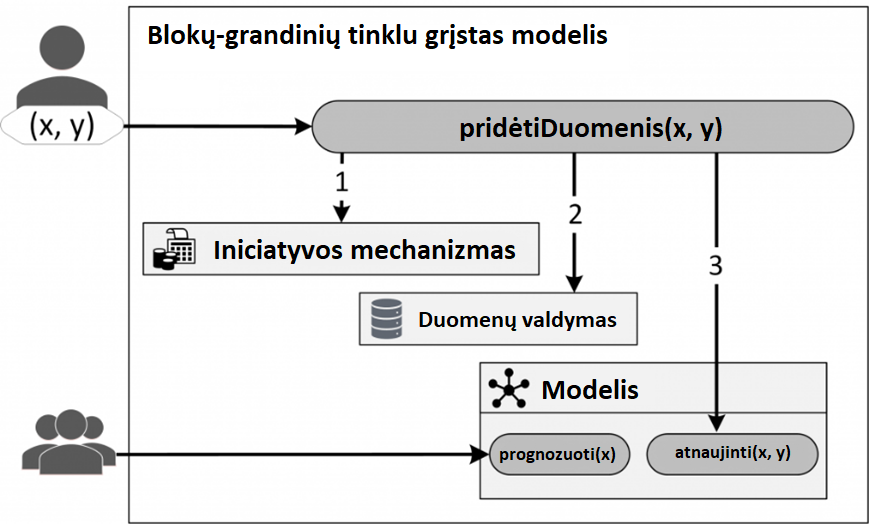
\includegraphics[width=9cm,height=6cm,keepaspectratio]{img/blockchain_1.png}
  \caption{Blokų-grandinių technologijų pritaikymas \cite{25}}
  \label{fig:Blokų-grandinių technologijų pritaikymas}
\end{figure}

\par Duomenų pridėjimas prie tinklo pavaizduotas pav. \ref{fig:Blokų-grandinių technologijų pritaikymas}. Procesas susideda iš trijų žingsnių \cite{25}:
\begin{itemize}
    \item Iniciatyvumo kūrimo mechanizmas. Jis skatina vartotojus teikti tik teisingus duomenis. Šiame žingsnyje pateikti duomenys yra validuojami, kaip transakcija. Iniciatyvumui gerinti yra daug būtų, vienas iš jų gali būti depozito sistema. Vartotojas pateikdamas duomenis tinklui, sumoka depozitą. Jeigu duomenys yra klaidinantys, depozitas nėra grąžinamas. Jeigu teisingi, depozitas grąžinamas ir, skatinimo tikslams, pridedama tam tikra suma. Duomenų teisingumas yra vertinamas pagal tai, kaip keičiasi modelio tikslumas su duotais duomenimis. Atitinkamai pagal modelio tikslumo pagerėjimą galima proporcingai vartotojui grąžinti daugiau pinigų.
    \item Duomenys yra siunčiami į blokų-grandinių tinklą ir ten pridedami. Pridėjus duomenis, visi vartotojai juos mato.
    \item Mašininio mokymosi modelis yra atnaujinamas pagal duomenis tinkle.
\end{itemize}
\par Esamas suprojektuotas karkasas geriausiai veikia tik nedideliems modeliams \cite{25}. Kol kas laukiama daugiau pasiūlymų, kaip būtų galima patobulinti blokų-grandinių technologijas, kad modelio mokymo procesas būtų efektyvesnis. Šiuo momentu pasiūlytas metodas neatsižvelgia į įrenginių ir duomenų heterogeniškumą, nėra efektyvaus mechanizmo nusakančio kaip tiksliai reikėtų apmokyti modelį su naujais duomenimis. Esantis sprendimas moko modelį su visais tinkle esančiais duomenimis. 

\subsection{Privatumo išsaugojimas}	
\par Pasiūlytas įmonės Microsoft sprendimas nėra saugus, nes kiekvieno vartotojo pateikti duomenys yra viešai matomi. Tačiau užtenka naudoti 4 skyriuje minimus homomorfinio šifravimo algoritmus ir problema yra išsprendžiama. Modelio saugumas tokiu atveju priklausytų tik nuo pasirinkto šifravimo algoritmo saugumo.
\par Lyginant su federuotu mokymosi algoritmu, pateiktas blokų-grandinių sprendimas išsprendžia kenkėjiškų įrenginių problemą. Pasiūlytame sprendime, prieš priimant vartotojo duomenis, jie yra įvertinami. Tačiau duomenų įvertinimui, į blokų-grandinių tinklą yra pridedama 10\% duomenų, validumo tikrinimo tikslams. \par Kadangi yra naudojami išmanieji kontraktai, šiuos duomenis galima bandyti iškarto pašalinti iš tinklo. Jeigu kenkėjiškas vartotojas bandytų apkrauti tinklą blogais duomenimis, jam tai daug kainuotų, nes kiekvieno tikrinimo atveju, jis neatgautų sumokėto depozito.
\parĮrenginių heterogeniškumo problema sprendime nėra sprendžiama ir duomenys yra lygiavertiškai imami iš visų įrenginių ir kiekvienas įrenginys gali vienodai prisidėti prie modelio kūrimo. Kadangi heterogeniškumas nėra tikrinimas, tinkle gali atsirasti daug duomenų, kurie turi labai mažą įtaką modelio tikslumui. Tai kainuoja daug skaičiavimo resursų modelio kūrimui.
\par Sprendžiant, kurį metodą pasirinkti, ar federuoto mokymosi, ar blokų-grandinių, reikia atsižvelgti į būsimo tinklo planuojamą dydį. Jeigu planuojama turėti daug įrenginių tinkle, blokų grandinių metodas yra geresnis, nes jis apsaugo nuo kenkėjiškų įrenginių. Jeigu tokių įrenginių būtų daug, iš surenkamo depozito būtų galima atitinkamai apdovanoti teigiamai tinklą paveikiančius naudotojus. Tačiau kadangi nėra atsižvelgiama į įrenginių ir duomenų galimą heterogeniškumą, prarandamas didelė dalis tinklo apmokymo efektyvumo. Jeigu vartotojų bus mažai blokų-grandinių tinkle, atsiranda rizika, jog tinklas nebus toks saugus ir ne visada jis bus prieinamas visiems vartotojams. Jeigu planuojama turėti nedaug vartotojų tinkle, federuotas mokymasis yra geresnis variantas. Kadangi yra vienas centralizuotas serveris, nėra problemų dėl tinklo pasiekiamumo, esant mažam skaičiui vartotojų. Analizuojant įrenginių ir duomenų heterogeniškumą, tinklas yra efektyvesnis apmokant modelį.  

\section{Saugus skirtingų pusių skaičiavimas}
\subsection{Apibrėžimas}
%https://eprint.iacr.org/2020/300.pdf%
\par Saugus skirtingų pusių skaičiavimo algoritmas („Secure Multiparty Computation“, trumpinys MPC) leidžia keliems įrenginiams skaičiuoti bendros funkcijos rezultatą, nesidalinant duomenimis tarpusavyje \cite{22}. Pagrindinis skirtumas, kuo  skiriasi MPC nuo kitų paskirstyto skaičiavimo algoritmų, yra didelis dėmesys saugumui. Kuriant MPC protokolą skaičiavimams atlikti, yra du reikalavimai: privatumas ir teisingumas. Privatumo reikalavimas reikalauja, kad įrenginiai, kurie vykdys skaičiavimus, sužinotų tik apskaičiuotą rezultatą ir nieko daugiau. Vienintelė papildomai sužinota informacija gali būti gauta tik išvedus ją iš gauto rezultato. Teisingumo reikalavimas reikalauja, kad kiekviena šalis turi gauti teisingai apskaičiuotą reikšmę. Jeigu vienas įrenginys apskaičiuos rezultatą klaidingai, visų įrenginių bendras skaičiavimo rezultatas bus irgi neteisingas. Paskirstyto skaičiavimo algoritmai irgi duotų neteisingą reikšmę, tačiau visų įrenginių bendras rezultatas nenukryptų daug.
\par Per laiką atsirado MPC protokolo patobulinimų, norint apsaugoti algoritmą nuo kenkėjiškų įrenginių, ir dėl to sukurti dar trys reikalavimai: įvesties duomenų nepriklausomumas, garantuotas reikšmės grąžinimas ir lygumas. Įvesties duomenų nepriklausomumo reikalavimas reikalauja, kad kiekvienas įrenginys nieko nežinotų apie kitų įrenginių naudojamus duomenis ir atitinkamai nekeistų savo duomenų. Garantuoto reikšmės grąžinimo reikalavimas reikalauja, kad kenkėjiški įrenginiai negalėtų sutrikdyti kitų įrenginių skaičiavimų. Pavyzdžiui, jeigu skaičiavimams naudojamas interneto ryšys, negali būti sudaryta galimybė leisti kenkėjiškiems įrenginiams paveikti interneto ryšio. Lygumo reikalavimas reikalauja, kad jeigu įrenginys turi blogus duomenis ar gautas rezultatas yra sugadintas, šis įrenginys turi gauti savo apskaičiuotą reikšmę tik tokiu atveju, jeigu visų kitų įrenginių rezultatai nėra sugadinti.
\subsection{Skaičiavimo algoritmai}
%https://ericrafaloff.com/shamirs-secret-sharing-scheme/%
\par MPC algoritmui paaiškinti, pirma reikia išsianalizuot atvejį, kai yra du įrenginiai su savo slaptais raktais ir viena paslaptis. Jeigu norime atgaminti paslaptį, reikia turėti abiejų įrenginių slaptus raktus ir taip galime atgaminti paslaptį. Pavyzdžiui, jeigu paslaptis yra skaičius 654321, tada reikia sugeneruoti atsitiktinį skaičių, kuris yra mažesnis už 654321. Tarkime tai yra 123456. Šis naujas atsitiktinis skaičiuos yra pirmo įrenginio slaptas raktas. Norint sukurti antro įrenginio raktą, galime iš slapto rakto atimti pirmo įrenginio raktą ir gauname 530865. Norint turėti daugiau įrenginių, kyla problema, kad siekiant atgaminti paslaptį, reikia visų įrenginių sutikimo. Jeigu vienas įrenginys bus prarastas, dings paslaptis. Tai nėra priimtinas sprendimas, todėl buvo sugalvotas algoritmas, kuris leidžia atgaminti paslaptį, turint tik dalį rakto dalių \cite{23}. Šis algoritmas vadinasi Shamir slapto rakto dalijimosi schema („Shamir‘s secret key sharing schema“), kitaip žinomas, kaip rakto skaldymo algoritmas. Slaptas raktas yra padalijamas yra kelias dalis. Kiekviena dalis pavieniui yra nepanaudojama. Slapto rakto atstatymui iš padalintų dalių, nebūtina turėti visas dalis. Pavyzdžiui, jeigu slaptas raktas yra padalijamas į penkias dalis, gali užtekti turėti tik tris dalis ir iš jų galima jau atstatyti pradinį slaptą raktą.
\par Shamir pasiūlė skaičiuoti slapto rakto dalis grafiškai 2D erdvėje \cite{23}. Paslaptis gali būti laikoma Y koordinate pradinio taško, kurio X koordinatė yra 0. Tada pasirenkame atsitiktinį tašką grafike ir brėžiame liniją tarp slapto taško ir atsitiktinai sugeneruoto taško. Tai grafiškai pavaidzuota pav. \ref{fig:Slapto rakto dalijimas tiesėje} Ši linija yra slapta ir ją žinant, galima atgaminti pradinę paslaptį. Kiekviena rakto dalis yra atsitiktinis taškas slaptoje linijoje. Turint dvi dalis, galima atgaminti slaptą raktą.  

\begin{figure}[ht]%
 \centering
 \subfloat[Slapto rakto dalijimas tiesėje]{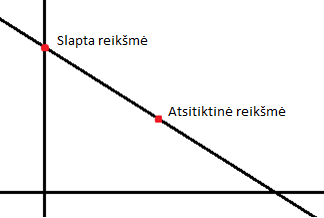
\includegraphics[width=9cm,height=6cm,keepaspectratio]{img/2ngraph.png}\label{fig:Slapto rakto dalijimas tiesėje}}%
 \subfloat[Slapto rakto dalijimas parabolėje \cite{24}]{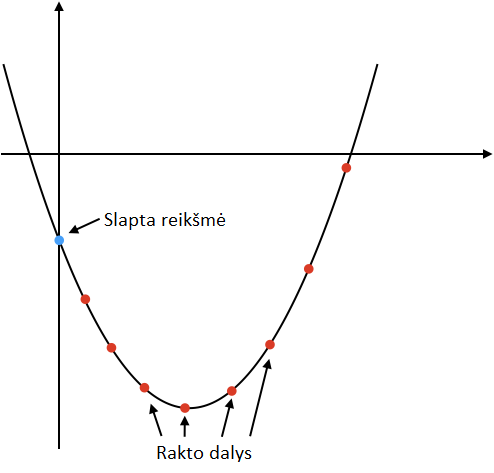
\includegraphics[width=9cm,height=6cm,keepaspectratio]{img/3ngraph.png}\label{fig:Slapto rakto dalijimas parabolėje}}%
 \caption{Slapto rakto dalijimas}%
 \label{fig:Slapto rakto dalijimas}%
\end{figure}

\par Norint leisti, kad paslaptį būtų galima atskleisti su dviem raktais, reikia sugeneruoti du atsitiktinius taškus ir nubrėžti slaptą parabolę \cite{23}. Turint tris sugeneruotus raktus, galima atkurti pradinę parabolės lygtį ir atkurti paslaptį. Rakto dalijimas grafiškai pavaizduotas pav. \ref{fig:Slapto rakto dalijimas parabolėje} Norint, kad paslaptis būtų atgaminta iš keturių raktų, reikia sugeneruoti kubinę kreivę ir taip toliau. %Panašus algoritmas yra  Reed-Solomon code.%

\section{Bendro įspūdžio privatus agregavimas}
\par Bendro įspūdžio privatus agregavimas, angliškai \say{Private Aggregation of Teacher Ensembles} (PATE), leidžia skirtingiems įrenginiams prisidėti prie bendro mašininio mokymosi modelių tinklo. Tinklą sudaro daug skirtingų mašininio mokymosi modelių, kurie nepriklausomai priima sprendimus. Kiekvieno modelio sprendimą tinklas susumuoja, pritaiko Gauso filtrą ir galutinį rezultatą pateikia vartotojui \cite{27}. Kiekvienas įrenginys turi galimybę pasirinkti savo mašininio mokymosi algoritmą ir realizuoti savo būdu, nepriklausomai nuo kitų įrenginių ar tinklo. Ši galimybė padaro tinklą efektyvesniu, nes įrenginiai gali pasirinkti algoritmus, kurie yra efektyvesni už tinko kūrėjo parinktą algoritmą.
\par Prieš kiekvienam įrenginiui pradedant kurti modelį, yra paskirstomi pagrindinio serverio privatūs duomenys dalimis \cite{27}. Kiekviena duomenų dalis neturi tokių įrašų, kurie kartojasi kitose dalyse. Kiekvienoje paskirstytoje dalyje kiekvienas įrašas yra unikalus. Jeigu su duotais duomenimis, tinklas išvedė teigiamą atsakymą, atsakyme negali būti atskleista jokia informacija apie pradinius privačius duomenis. Tai yra todėl, nes jeigu du modeliai priima bendrą sprendimą apie duomenis ir tik vienas modelis galėjo būti apmokytas su tokiais duomenimis, antro modelio išvestis yra nepriklausoma nuo jo pradinių duomenų. 
\par Vienintelis būdas gauti informacijos apie modelių pradinius duomenis yra analizuoti bendrą tinklo išvestį ir tikrinti kiek kokių modelių ką išvedė. Dėl šios priežasties, PATE tinklas naudoja Gauso filtrą, prieš pateikiant galutinę išvestį \cite{27}. Gauso filtras paprastai yra naudojamas vaizdų suliejimui, detalių panaikinimui \cite{28}. Modelių \say{balsų} skaičiavimui, naudojamas Gauso 1D filtras. Gauso filtro skaičiavimas pateiktas lygtyje \eqref{eq:Gauso filtras}. 

\begin{equation}
    G(x) = \frac{1}{\sqrt{2 \cdot \pi \cdot \sigma^{2}}}e^{-\frac{x^{2}}{2 \cdot \sigma^{2}}}
    \label{eq:Gauso filtras}
\end{equation}

Čia $\sigma$ yra standartinis skirstinio nuokrypis. 
\par Dabar PATE tinkle atsiranda dvi problemos \cite{27}. Pirma problema atsiranda, kai vykdoma daug užklausų ir jos yra panašios. Tokiu atveju, galima atgaminti informaciją apie pradinius duomenis analizuojant tinklo skirtingas išvestis su panašiais duomenimis. Dėl šios problemos reikėtų riboti galimą užklausų skaičių kiekvienam tinklo naudotojui. Skaičiui pasiekus ribą, reikia gauti naujus duomenis ir sukurti naujus modelius su šiais duomenimis. Antra, tinklas turi daug skirtingų modelių ir dėl to negalima paviešinti tinklo, kaip vieno modelio. Taip yra daroma, norint apsisaugoti nuo pradinių parametrų atgaminimo. Dėl šių problemų, PATE tinklas turi papildomą žingsnį: studento modelio kūrimas. Studento modelis yra apmokomas, perkeliant visų sukurtų modelių tinkle parametrus į vieną. Tai yra atliekama naudojant viešus nesurūšiuotus duomenis ir juos leidžiant pro tinklą. Susumavus visų tinklo modelių \say{balsus}, jie yra filtruojami su Gauso filtru. Galutinis rezultatas yra naudojamas mokant studento modelį. Šis studento modelis yra galutinis PATE tinklo rezultatas.
\par PATE galima patobulinti keliais būdais:
\begin{itemize}
    \item Serveris, kuris paskirsto duomenis į dalis, turėtų naudoti homomorfinį šifravimą, prieš atiduodant duomenis kitiems įrenginiams. Tai netik paslėptų duomenis nuo modelių kūrėjų ir pašalintų duomenų nutekėjimo riziką, bet ir padarytu pačius modelius ir visą tinklą saugesnį.
    \item Kuriant studento modelį, turi būti atliekama kiek galima mažiau užklausų į bendrą modelių tinklą \cite{26}. Pavyzdžiui, užklausos turi būti atliekamos tik iki tol, kol pasiekiamas studento modelio tam tikras tikslumas. Taip pat užklausos turi būti atliekamos su nepanašiais duomenimis. Kuo daugiau yra atliekama užklausų į bendrą modelių tinklą ir kuo jos yra panašesnės, tuo labiau yra tikėtina, kad bus galima atskleisti pradinius modelių duomenis.
    \item Norint turėti optimalų privatumo išsaugojimą, tinkle esantys modeliai turėtų grąžinti panašius rezultatus \cite{26}. Jeigu keli modeliai išsiskiria rezultatais nuo kitų modelių tinkle, atsiranda tikimybė, kad bus atskleisti pradiniai modelių duomenys. Tai gali nutikti kaip bus siunčiama daug panašių užklausų ir gausis skirtingi rezultatai. Panašus eksperimentas, kuris veiktų ir su PATE tinklu, siekiant atskleisti pradinius duomenis, yra atliktas 3.3 skyriuje. Pavyzdyje yra naudojami kiti algoritmai, tačiau PATE tinklo pažeidžiamumo esmė yra tapati.
\end{itemize}

\par Lyginant PATE algoritmą su federuotu mokymu, PATE yra saugesnis, nes tinkle modelių yra nors keli ir jeigu duoti duomenys yra panašūs į vieno modelio pradinius duomenis, esant bendram modelių sutarimui, sunku atgaminti pradinius duomenis, iš tinklo išvesties. Pradinių duomenų atgaminimą taip pat apsunkina ir Gauso filtras. Optimaliu atveju, privatumas tinkle yra geriausiai išsaugomas, kai kiekvienas modelis grąžina panašius rezultatus su duotais viešais duomenimis, tada negalima atsekti kuris modelis tinkle yra už tai atsakingas. PATE yra taip pat ir efektyvesnis už federuotą mokymą, nes modelius kuria įrenginiai, kurie gali pasirinkti tam tikrai duomenų sričiai optimalius algoritmus, o federuotas mokymas apibrėžia tik vienodų algoritmų naudojimą. PATE taip pat išsprendžia įrenginių ir duomenų heterogeniškumo problemas. Vienintelis federuoto mokymosi pranašumas yra, kad nereikia dalintis pradiniais duomenimis. Jeigu jie yra svarbūs, o įrenginiai nėra patikimi, atsiranda rizika, kad įrenginiai gali atskleisti duomenis. Tačiau ši problema gali būti išspręsta su 4 skyriuje minimais šifravimo algoritmais, kurie leistų paslėpti duomenis nuo pačių įrenginių.

\section{Tensorflow karkasas}
\par \say{Tensorflow} karkasas - Google technologijų įmonės atviro kodo, mašininio mokymosi karkasas. Šiame karkase yra realizuota daug algoritmų ir mašininio mokymosi modelių. 2019 metais kovo mėnesį \say{Tensorflow} karkaso puslapyje buvo pristatytas straipsnis apie diferencinį privatumą. Prie \say{Tensorflow} karkaso buvo pridėta Tensorflow Privacy biblioteka, kuri realizuoja mašininio mokymosi modelius, naudojančius diferencinį privatumą \cite{29}. Iki to laiko, \say{Tensorflow} karkasas neatsižvelgdavo į duomenų išsaugojimą. 4 skyriuje aprašytus homomorfinio šifravimo algoritmus nebuvo galima taikyti karkase. Vienintelis būdas išsaugoti privatumą buvo naudoti skirtingų mašininių modelių tinklą, pavyzdžiui 5 skyriuje aprašytą federuotą mašininį mokymąsi arba 8 skyriuje aprašytą bendro įspūdžio agregavimo algoritmą.
\par Atsitiktinai parinktos reikšmės $M : D $\rightarrow$ R$ tenkina diferencinio privatumo sąlygą, kai du duomenų rinkiniai $X ir X' \in D$, išvestys $\Upsilon \in R$ ir tenkinama sąlyga lygybėje \ref{eq:Diferencinio privaluto sąlyga} \cite{30}. Čia $Pr[X]$ - tikimybė, kad įvyks įvykis $X$. Ši sąlyga užtikrina, kad parinkti du duomenų rinkiniai $X$ ir $X'$, kurie skiriasi tik vienu įrašu, duos labai panašius rezultatus, kurių neis atskirti. Šioje lygtyje $\epsilon$ yra vadinamas privatumo biudžetu - kuo mažesnis yra $\epsilon$, tuo gaunamas didesnis duomenų saugumas.

\begin{equation}
    Pr[M(X) \in \Upsilon] \leq e^{\epsilon} Pr[M(X') \in \Upsilon] + \delta
    \label{eq:Diferencinio privaluto sąlyga}
\end{equation}

\par Pagrindinė pasiūlyto algoritmo idėja - vykdant stochastinio gradiento nuolydžio algoritmą, modifikuoti gradientų reikšmes. Tai yra atliekama su dviem algoritmo pakeitimais:

\begin{itemize}
    \item Kiekvieno gradiento jautrumas pokyčiams turi būti apribotas. Reikia nurodyti, kiek kiekviena duomenų eilutė gali paveikti kiekvieną gradientą. Šiam tikslui yra taikoma procedūra \say{Clipping}, kuri nusako maksimalų galimą gradientų pokytį.
    \item Siekiant išsaugoti privatumą, pridedamas triukšmas prie reikšmės, gautos iš \say{Clipping} metodo. Triukšmas yra gaunamas su Gauso filtru. Taikant filtrą nustatomos ir apribojamos reikšmės kiekvienam gradientui atsitiktinai, taip išsaugomas privatumas
\end{itemize}

\par \say{Tensorflow Privacy} leidžia saugumo prasme optimizuoti modelį, nekuriant jo iš naujo ir nekeičiant pradinių modelio parametrų. Tai yra verslui geras sprendimas, nes kuriant sprendimą yra daugiausiai skiriama dėmesio į modelio tikslumą ir mažai investuojama laiko galvojant apie modelio saugumą. Šį funkcionalumą atlieka du paketai esantys \say{Tensorflow Privacy} karkase. Vienas iš jų yra \say{Bolt-on} paketas, kuris modifikuoja sukurtą modelį prieš jo naudojimą gamybinėje aplinkoje. Jis prie kiekvieno modelio svorio prideda triukšmo.

\section{Tyrimas}
\subsection{Modelių palyginimas}

\par Tyrimo tikslams, buvo sukurti modeliai ir, skaičiuojant DMDK metriką, jie lyginami tarpusavyje. Tyrimui paimti diabetu sergančių žmonių duomenys iš \say{Sklear} bibliotekos viešai prieinami duomenys. Gauti rezultatai pateikti lentelėje \ref{tab:DMDK rezultatai}.

\begin{table}[h]
\begin{adjustbox}{width=\textwidth,center=\textwidth}
\begin{tabular}{|l|l|l|l|}
\cline{1-4}
Modelis & Nuostolių f-jos reikšmė (MSE) & Tikslumas & DMDK  \\\cline{1-4}
PyTorch neuroninis tinklas & 103.9837813 & 81.1\% & 87.419  \\\cline{1-4}
Gradientinio nuolydžio algoritmas & 2272.06 & 63.78\% & 0.051792 \\\cline{1-4}
Pallier homomorfiniu šifravimu grįstas modelis & 2185.37 & 63.52\% & 0.1416 \\\cline{1-4}
\end{tabular}
\end{adjustbox}
\caption{Sugalvotos duomenys reikšmės modelio tikrinimui}
\label{tab:DMDK rezultatai}
\end{table}

\par Pagal gautus rezultatus, pateiktus lentelėje \ref{tab:DMDK rezultatai}, gautos išvados:
\begin{itemize}
    \item PyTorch neuroninis tinklas greičiau artėja prie nuostolių funkcijos minimumo, nei kiti modeliai. Esant ~70\% modelių tikslumui, PyTorch modelis yra saugiausias. Mažiausiai saugus yra paprastu gradientiniu nuolydžiu grįstas modelis. 
    \item Palliers kriptografija grįstas modelis yra saugesnis už paprastą gradientinio nuolydžio metodą.
    \item Didėjant PyTorch modelio tikslumui, jis pradeda labiau prisirišti prie duomenų ir vidutinė galima maksimalaus nuokrypio reikšmė smarkiai krenta – modelis tampa vis mažiau saugus. Jeigu uždavinio tikslas yra sukurti labai tikslų modelį, vertėtų apgalvoti ar Pallier sistema grįstas modelis nėra geriau.
    \item Su visais modeliais, išskyrus PyTorch neuroninį tinklą, didėjant modelio tikslumui, didėja vidutinė maksimalaus nuokrypio reikšmė – modelis tampa saugesnis, o su PyTorch neuroniniu tinklu, mažėja - modelis tampa mažiau saugus. 
\end{itemize}

\par Tas pats tyrimas buvo atliktas su MNIST rašytinių skaitmenų nuotraukomis. Tik PyTorch neuroninis tinklas su vienu paslėptu sluoksniu ir VGG16 konvergavo minimumo link. Pasiekus 74\% ir 82\% tikslumus, PyTorch neuroninio tinklo DMDK reikšmės išlieka vienoda - 0.04999, MSE nuostolių funkcijos reikšmės atitinkamai 266.66730 ir 203.6602. VGG16 tinklui pasiekus 72\% tikslumą, MSE nuostolių funkcijos reikšmė - 2.59, DMDK reikšmė -  0.17. Reiškia VGG16 modelis yra saugesnis už paprastą vieno paslėpto sluoksnio PyTorch neuroninį tinklą.

\par Kiekvienam modeliui atliktas atskiras nuostolių funkcijos (MSE), DMDK rodiklių ir modelio tikslumo, DMDK priklausomybės tyrimas.

\subsubsection{Pallier homomorfiniu šifravimu grįsto modelio detalus tyrimas}
\par DMDK rodiklio reikšmių priklausomybė nuo MSE nuostolių funkcijos reikšmių pateikta pav. \ref{fig:Palliers DMDK rodiklio reikšmių priklausomybė nuo MSE nuostolių funkcijos reikšmių}. Čia X ašis - MSE nuotolių funkcijos reikšmės, Y ašis - DMDK reikšmės. 

\begin{figure}[h]
  \centering
  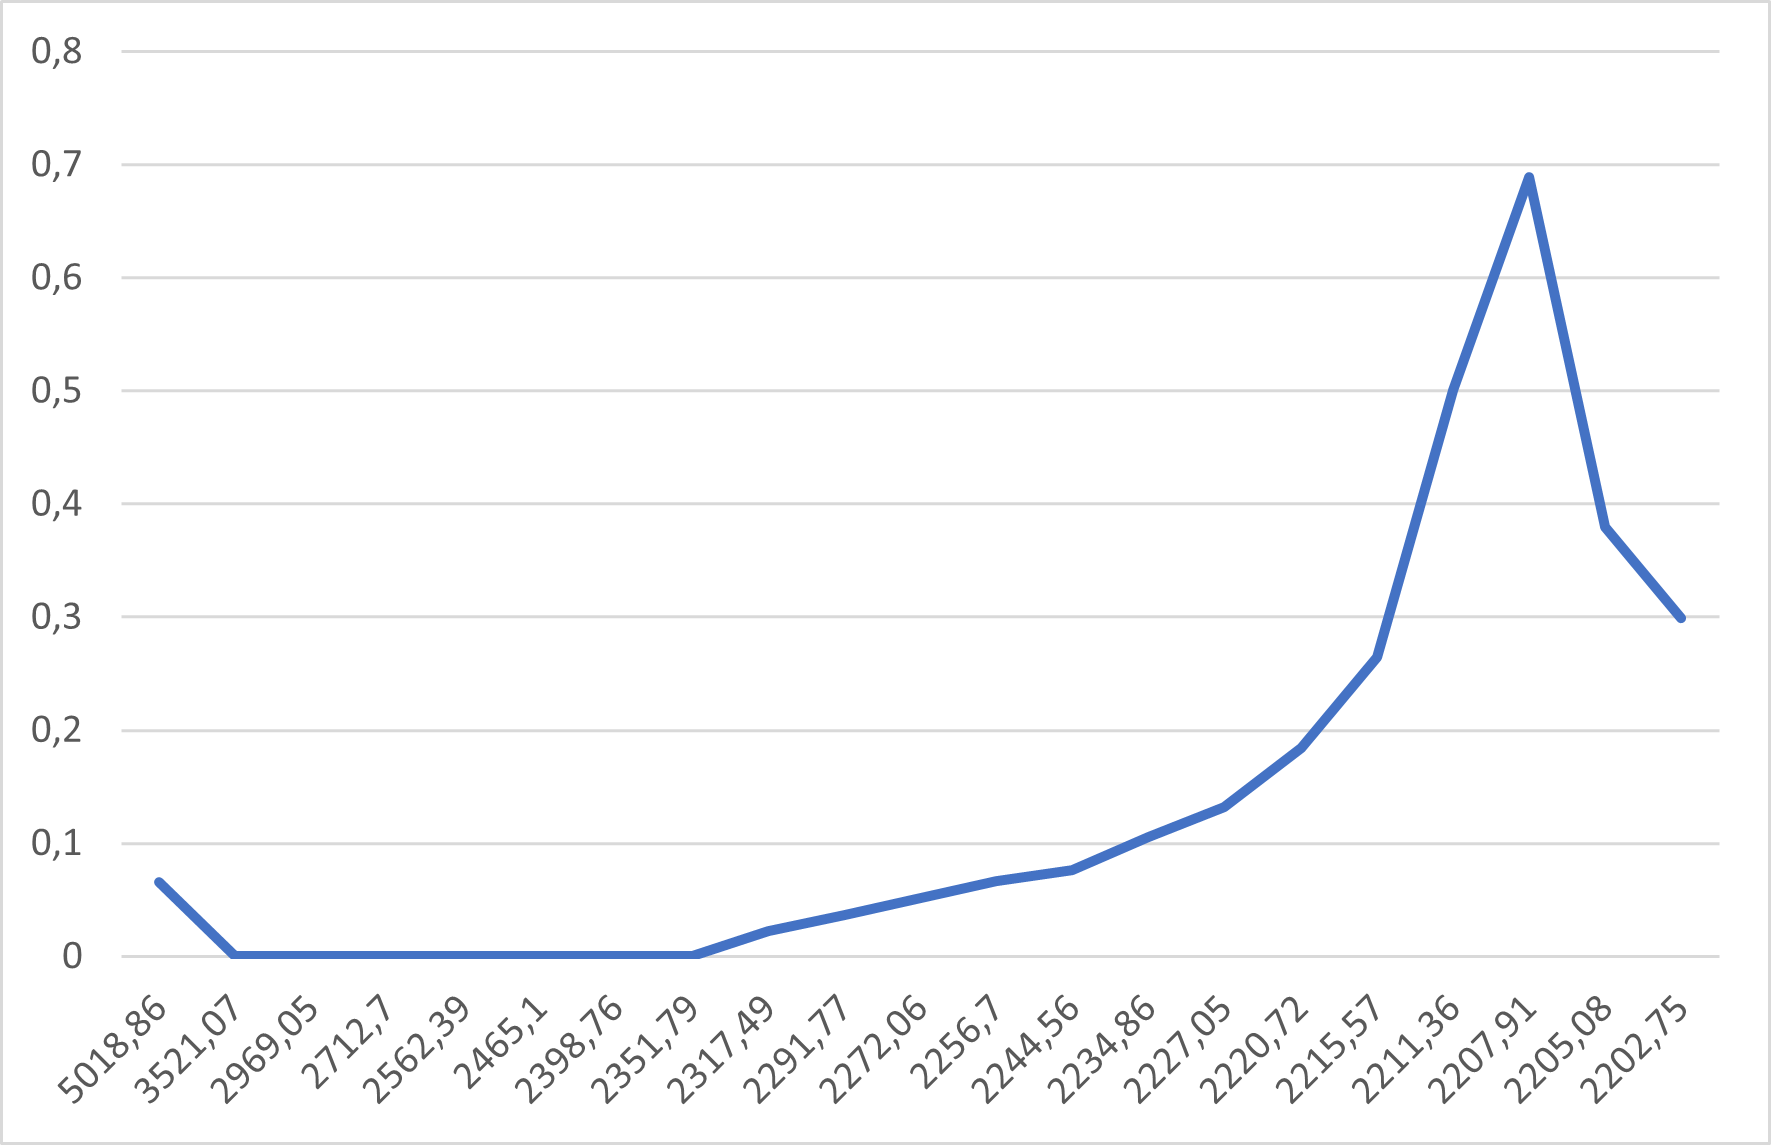
\includegraphics[width=14cm,height=11cm,keepaspectratio]{img/pal_tyr_1.png}
  \caption{Palliers DMDK rodiklio reikšmių priklausomybė nuo MSE nuostolių funkcijos reikšmių}
  \label{fig:Palliers DMDK rodiklio reikšmių priklausomybė nuo MSE nuostolių funkcijos reikšmių}
\end{figure}

\par DMDK rodiklio reikšmių priklausomybė nuo modelio tikslumo pateikta pav. \ref{fig:Palliers DMDK rodiklio reikšmių priklausomybė nuo MSE nuostolių funkcijos reikšmių}. Čia X ašis - modelio tikslumas procentais, Y ašis - DMDK reikšmės.

\begin{figure}[h]
  \centering
  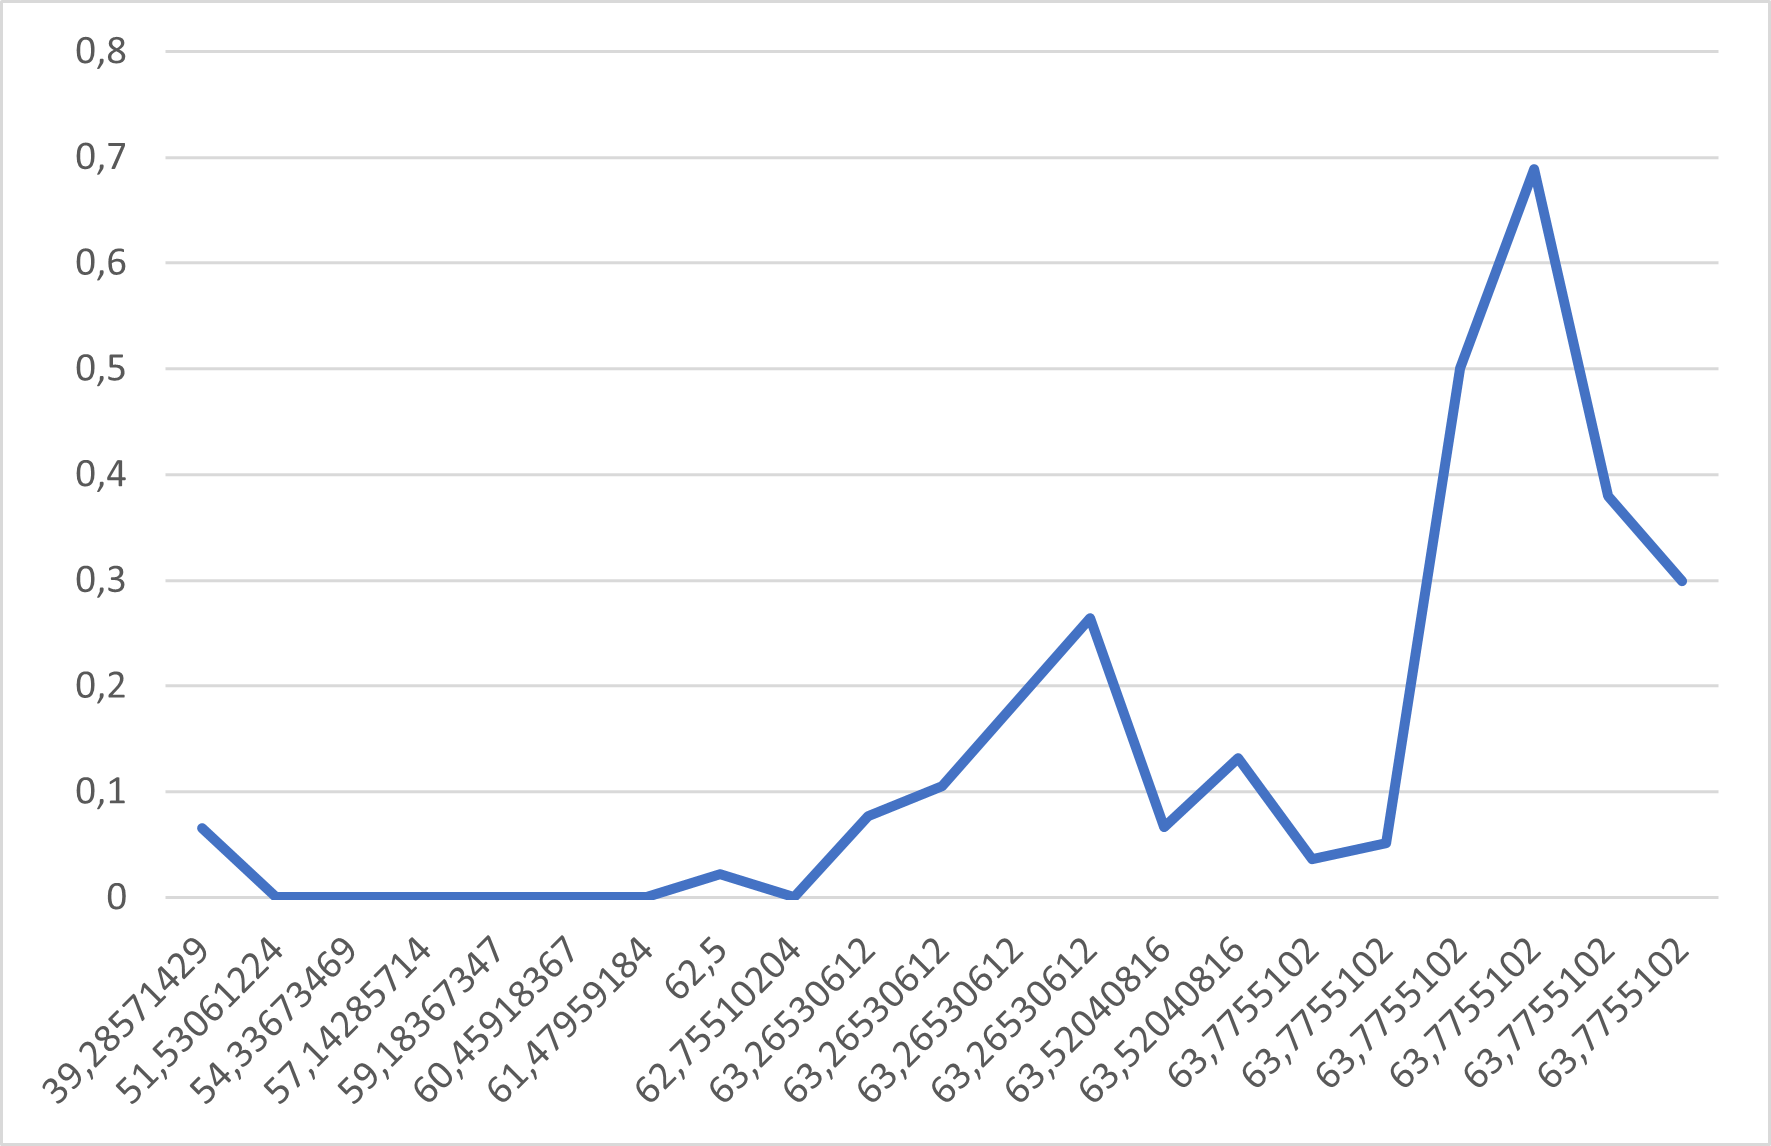
\includegraphics[width=14cm,height=11cm,keepaspectratio]{img/pal_tyr_2.png}
  \caption{Palliers DMDK rodiklio reikšmių priklausomybė nuo MSE nuostolių funkcijos reikšmių}
  \label{fig:Palliers DMDK rodiklio reikšmių priklausomybė nuo MSE nuostolių funkcijos reikšmių}
\end{figure}

\par Iš atlikto tyrimo matosi koreliacija tarp modelio nuostolių funkcijos reikšmių ir DMDK reikšmių. Kuo nuostolių funkcijos reikšmė yra mažesnė, tuo DMDK yra didesnis ir modelis yra laikomas saugesnis. Vietos, kuriose DMDK yra lygus 0, modelis yra per daug prisirišęs prie parametrų. DMDK tiesioginės priklausomybės nuo modelio tikslumo, neturi.

\subsubsection{PyTorch neuroninio tinklo detalus tyrimas}
\par DMDK rodiklio reikšmių priklausomybė nuo MSE nuostolių funkcijos reikšmių pateikta pav. \ref{fig:PyTorch neuroninio tinklo DMDK rodiklio reikšmių priklausomybė nuo MSE nuostolių funkcijos reikšmių}. Čia X ašis - MSE nuotolių funkcijos reikšmės, Y ašis - DMDK reikšmės. 

\begin{figure}[h]
  \centering
  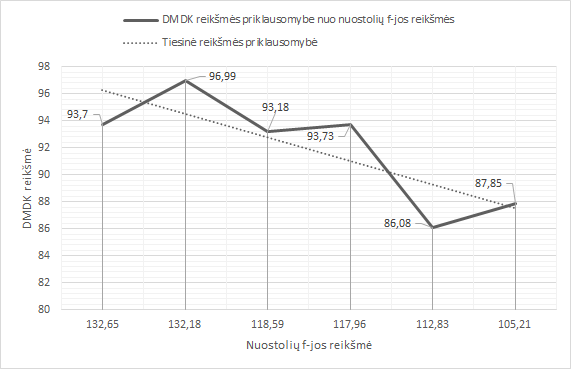
\includegraphics[width=11cm,height=8cm,keepaspectratio]{img/pap_tyr_1.png}
  \caption{PyTorch neuroninio tinklo DMDK rodiklio reikšmių priklausomybė nuo MSE nuostolių funkcijos reikšmių}
  \label{fig:PyTorch neuroninio tinklo DMDK rodiklio reikšmių priklausomybė nuo MSE nuostolių funkcijos reikšmių}
\end{figure}

\par DMDK rodiklio reikšmių priklausomybė nuo modelio tikslumo pateikta pav. \ref{fig:PyTorch neuroninio tinklo DMDK rodiklio reikšmių priklausomybė nuo MSE nuostolių funkcijos reikšmių}. Čia X ašis - modelio tikslumas procentais, Y ašis - DMDK reikšmės.

\begin{figure}[h]
  \centering
  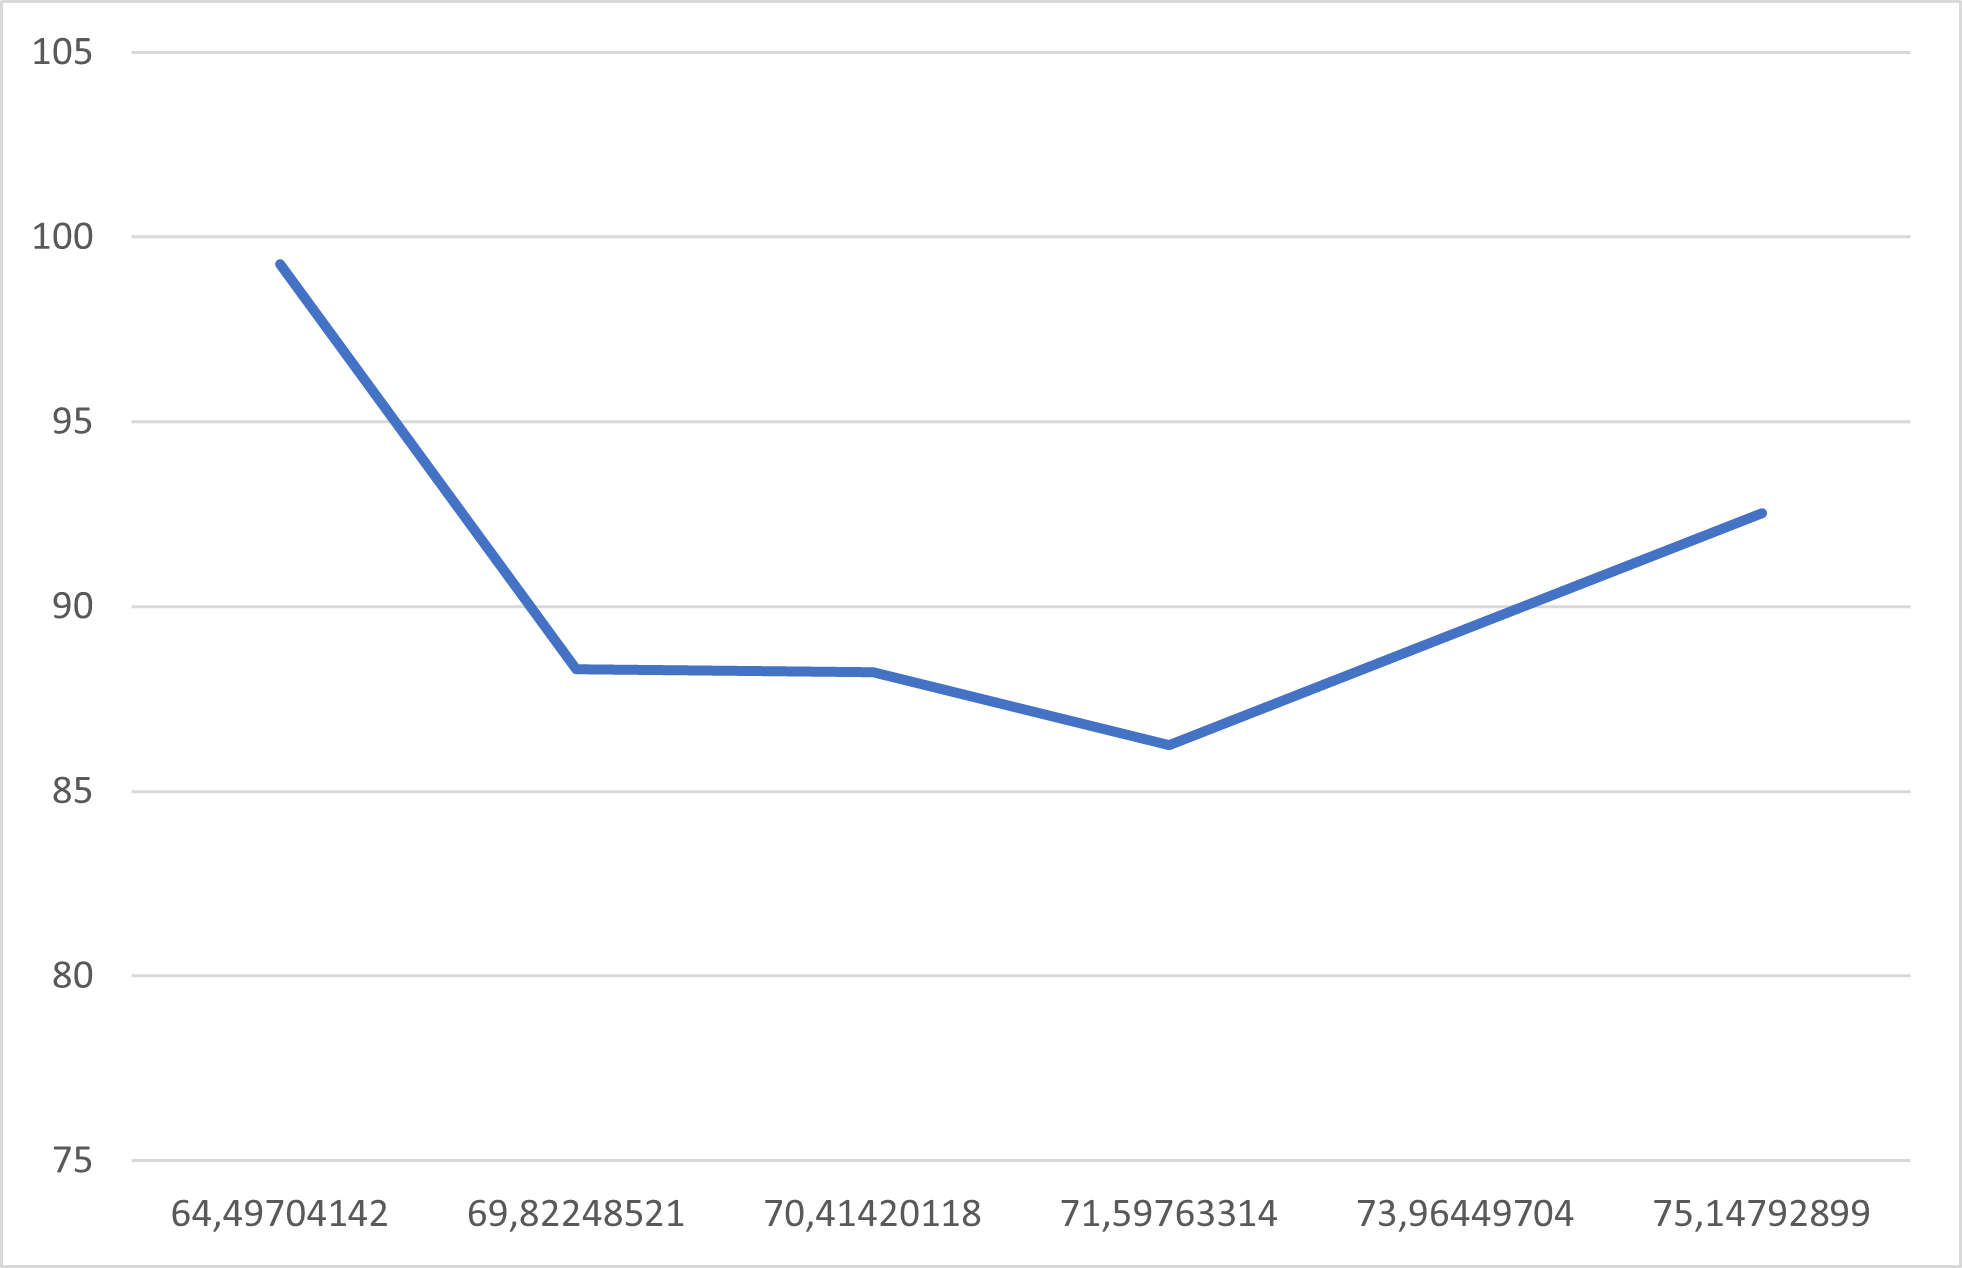
\includegraphics[width=11cm,height=8cm,keepaspectratio]{img/pap_tyr_2.png}
  \caption{PyTorch neuroninio tinklo DMDK rodiklio reikšmių priklausomybė nuo MSE nuostolių funkcijos reikšmių}
  \label{fig:PyTorch neuroninio tinklo DMDK rodiklio reikšmių priklausomybė nuo MSE nuostolių funkcijos reikšmių}
\end{figure}

\par Iš atlikto tyrimo nesimato jokios stiprios koreliacijos tarp DMDK rodiklio ir MSE nuostolių funkcijos reikšmių ar modelio tikslumo.

\subsection{Duomenų triukšmo įtakos tyrimas}

\par Atliktas tyrimas su PyTorch 3-jų sluoksnių neuroniniu tinklu ir duomenų triukšmu. Modelis kiekvieno bandymo metu atlieka 250 iteracijų. Kiekvieną kartą kai yra nuskaitomi duomenys, pridedamas atsitiktinis triukšmas, kuris neviršija nurodytos reikšmės. Tyrime buvo keičiamas maksimalus generuojamas duomenų triukšmas ir stebima, kokią įtaką tai turi sukurtam modeliui.
\par Tyrime pastebėta, kad tarp triukšmo ir modelio duomenų saugumo rodiklio DMDK yra koreliacija, kuri matoma pav. \ref{fig:DMDK priklausomybė nuo pridėto triukšmo}. Didinant atsitiktinį duomenų triukšmą, gerėja modelio duomenų saugumas. Pastebėta taip pat ir koreliacija tarp modelio tikslumo ir pridėto triukšmo prie duomenų. Pav. \ref{fig:Modelio tikslumo priklausomybė nuo pridėto triukšmo} parodyta, kad didinant modelio duomenų triukšmą, mažėja modelio tikslumas.

\begin{figure}[h]
  \centering
  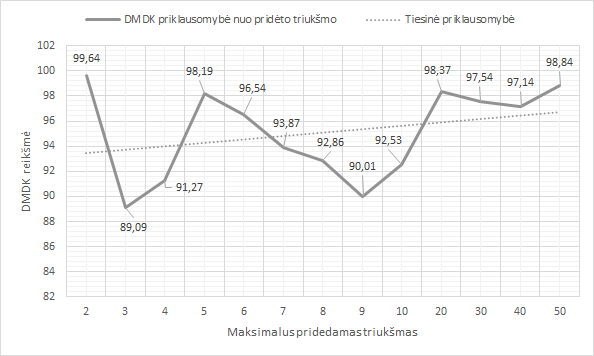
\includegraphics[width=13cm,height=9cm,keepaspectratio]{img/tr_tyr_dmdk.png}
  \caption{DMDK priklausomybė nuo pridėto triukšmo}
  \label{fig:DMDK priklausomybė nuo pridėto triukšmo}
\end{figure}

\begin{figure}[h]
  \centering
  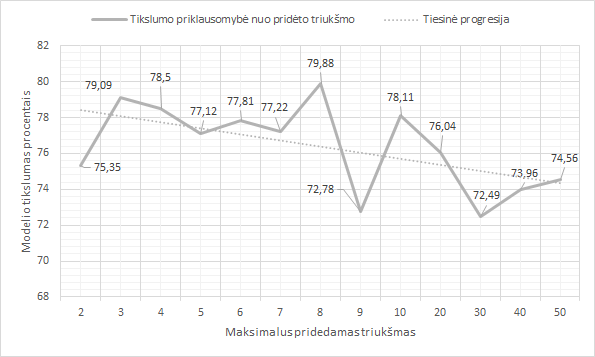
\includegraphics[width=13cm,height=9cm,keepaspectratio]{img/tr_tyr_acc.png}
  \caption{Modelio tikslumo priklausomybė nuo pridėto triukšmo}
  \label{fig:Modelio tikslumo priklausomybė nuo pridėto triukšmo}
\end{figure}

\subsection{Duomenų kiekio ir DMDK tyrimas}
\par Buvo atliktas bandymas generuoti duomenis ir tikrinti, kaip keičiasi DMDK reikšmė kintant duomenų kiekiui. Tyrimas buvo atliekant generuojant duomenis panašius į esančius Sklearn žmonių sergančiu cukriniu diabetu, duomenų rinkinyje. Tiriant nebuvo rasta koreliacija tarp sugeneruoto duomenų kiekio ir DMDK reikšmės. Tai reiškia, kad didinant pradinių duomenų kiekį, modelio saugumas nekinta.

\subsection{Tyrimo išvados}

\begin{itemize}
    \item Lyginant PyTorch neuroninį tinklą, paprastą gradientinio nuolydžio algoritmą ir Pallier homomorfiniu šifravimu grįstą modelį, jeigu visi minėti modeliai vykdant tyrimą konverguoja minimumo link, pats saugiausias modelis yra PyTorch neuroninis modelis. Mažiausiai duomenis saugantis yra paprastas gradientinis metodas.
    \item Naudojant Pallier homomorfiniu šifravimu grįstą modelį, egzistuoja koreliacija tarp modelio nuostolių funkcijos reikšmės ir DMDK rodiklio. Vidutiniškai, kuo nuostolių funkcijos reikšmė yra mažesnė, tuo DMDK rodiklis yra didesnis ir modelis yra saugesnis.
    \item Pallier homomorfiniu šifravimu grįstas modelis, naudojantis gradientinio nuolydžio algoritmą, diverguoja su MNIST rašytinių skaičių nuotraukomis.
    \item Paprastas PyTorch neuroninis tinklas vienintelis iš minėtų modelių konverguoja minimumo link, su MNIST rašytinių skaičių nuotraukomis. Šiuo atveju, DMDK rodiklis vidutiniškai nukrenta iki 0.049 ir modelis tampa mažiau saugus, nei Pallier algoritmu grįstas modelis.
    \item Didinant duomenų triukšmą, didėja DMDK reikšmė ir modelis tampa saugesnis, tačiau sumažėja modelio tikslumas.
    \item Pradinių duomenų kiekis neturi įtakos modelio duomenų saugumui.
\end{itemize}

\section{Išvados}
\par Darbe buvo išanalizuoti algoritmai, kurie yra skirti duomenų privatumo išsaugojimui mašininiame mokymesi.  Darbe buvo realizuotas vienas iš homomorfinio šifravimo algoritmų - Paillier sistema. Atlikti saugumo tyrimai parodė, kad naudojant gradientinį nuolydį ir Paillier sistemą, pradiniai modelio duomenys yra saugesni, nei tik naudojant gradientinį nuolydį be jokio šifravimo. Nustatyta, kad modelio tikslumui artėjant 100\%, greitai kyla ir DMDK reikšmė. Tai reiškia, kad modelio pradiniai duomenys tampa saugesni. Planuojant, kad modelio tikslumas bus arti 100\%, modelio duomenų saugumui pagerinti reikia naudoti homomorfinį šifravimą.
\par Buvo atliktas duomenų saugumo tyrimas su PyTorch 3-jų sluoksnių neuroniniu modeliu. Analizuojant Sklearn bibliotekoje esančius cukriniu diabetu sergančių žmonių duomenis, paaiškėjo, kad PyTorch neuroninis modelis yra ~20 kartų saugesnis nei Paillier kriptogravifos taikymas su gradientiniu nuolydžio algoritmu. Pastebėta tendencija, kad modelio tikslumui artėjant 100\%, mažėja DMDK reikšmė ir modelis tampa mažiau saugus. Jis labiau prisiriša prie pradinių duomenų ir linksta link jų atskleidimo. Planuojant, kad modelio tikslumas nebus didelis ir siek tik ~60\% tikslumą, reiktų apsvarstyti homomorfinio šifravimo saugumą su tokiu uždaviniu.
\par Minėtas PyTorch tyrimas su cukriniu diabetu sergančiais duomenimis parodė, kad esant ~15 parametrų, modelis yra saugesnis už homomorfinį šifravimą. Kitas atliktas tyrimas buvo su MNIST duomenų rinkiniu. Šiame rinkynyje yra ranka rašyti skaitmenys. Esant dideliam modelio paramentrų skaičiui, PyTorch prarado savo pradinių duomenų saugumą, jis tapo mažesnis už Paillier kriptografijos saugumą. Esant didesniam parametrų skaičiui, PyTorch 3-jų sluoksnių modelis yra labiau linkęs \say{prisirišti} prie pradinių duomenų. Prieš kuriant modelį ir pasirenkant algoritmą reikia apsvarstyti kokio tikslumo modelio galima tikėtis gauti ir kiek parametrų modelis priims, nes nuo to priklauso ar naudoti neuronininus tinklus ar homomorfinį šifravimą.
\par Kitame tyrime pastebėta koreliacija tarp modelio saugumo metrikos DMDK ir pridedamo triukšmo. Kuo pridedamas triukšmas yra didesnis, tuo DMDK metrika yra didesnė ir modelio pradiniai duomenys yra saugesnis, tačiau didinant pridedamą triukšmą, mažėja modelio tikslumas. Planuojant, kad bus naudojami neuroniniai tinklai be homomorfinio šifravimo ir tikimasi didesnio nei 80\% modelio tikslumo, vertėtų pridėti triukšmą prie pradinių modelio duomenų.

%\printbibliography[heading=bibintoc]
\bibliographystyle{alpha}
\bibliography{bibliografija}

\end{document}